\documentclass[10pt,a4paper]{article}

% Packages indispensables
\usepackage[utf8]{inputenc}
\usepackage[T1]{fontenc}
\usepackage[french]{babel} % Pour la typographie française
\usepackage{amsmath, amssymb, amsthm} % Pour les mathématiques
\usepackage{graphicx} % Pour insérer des images/graphiques
\usepackage{hyperref} % Pour les liens cliquables
\usepackage{geometry} % Pour gérer les marges
\usepackage{booktabs} % Pour faire de jolis tableaux
\usepackage{caption}
\usepackage{subcaption} % Pour mettre plusieurs figures côte à côte
\usepackage{microtype}
\usepackage{float}

\setlength{\parskip}{4pt}\setlength{\parindent}{0pt}

\linespread{1.05}

% Réglage des marges
\geometry{
    top=2cm,
    bottom=2cm,
    left=2.5cm,
    right=2.5cm,
    columnsep=0.8cm
}

% Informations du document
\title{\textbf{Analyse et Benchmarking d'Algorithmes de Descente}\\ \vspace{3mm} \large{OCVX1}}
\author{
    @KadirKess
    \and 
    @sachaMelin
    \and 
    @valentin-best
}
\date{}

\begin{document}

\maketitle

\begin{abstract}
\noindent Ce rapport présente une étude empirique de différents algorithmes d'optimisation. Plutôt que de prouver l'exactitude des implémentations, notre démarche se concentre sur l'analyse de la sensibilité de ces algorithmes face aux variations d'hyperparamètres et aux conditions initiales. À travers trois benchmarks, nous mettons en perspective nos résultats expérimentaux avec les garanties théoriques étudiées en cours.
\end{abstract}

\tableofcontents

\newpage

\section*{Introduction}
L'optimisation numérique joue un rôle central dans de nombreux domaines scientifiques. S'il est aisé d'implémenter des algorithmes de descente, évaluer leur robustesse et leur efficacité requiert une méthodologie rigoureuse. 

L'objectif de ce document est de présenter trois études ciblant différents aspects des méthodes de descente~:
\begin{itemize}
    \item \textbf{Benchmark 1~:} Influence conjointe des deux hyperparamètres du critère d'Armijo dans le cas d'une descente de gradient.
    \item \textbf{Benchmark 2~:} Influence du choix de la méthode (Fletcher-Reeves contre Polak-Ribière) dans l'algorithme du gradient conjugué sur une classe de fonctions non-convexes.
    \item \textbf{Benchmark 3~:} Comparaison de rapidité et de précision pour les méthodes de gradient conjugué, Newton (dans le cas quadratique) et quasi-Newton dans le cas général.
\end{itemize}


\section{Cadre de l'étude}

\subsection{Fonctions test}\label{sec:fonctions}

Quatre familles de fonctions sont utilisées dans l'ensemble des benchmarks.

\textbf{Fonction quadratique convexe.} Pour $A \in \mathbb{R}^{n \times n}$ symétrique définie positive et $b \in \mathbb{R}^n$~:
\[
  f_Q(x) = \tfrac{1}{2}x^\top A x - b^\top x.
\]
Le minimum global est $x^\star = A^{-1}b$, connu analytiquement, ce qui permet de mesurer l'erreur exacte $\|x_k - x^\star\|_2$. Le conditionnement $\kappa(A)$ est le principal levier de difficulté.

\textbf{Fonction de Rosenbrock.} Fonction non-convexe classique sur $\mathbb{R}^2$~:
\[
  f_R(x) = (x_1 - 1)^2 + \gamma(x_1^2 - x_2)^2,
\]
dont le minimum global $x^\star = (1,1)$ se situe au fond d'une vallée parabolique étroite. Le paramètre $\gamma$ contrôle le rapport d'aspect de la vallée et donc la difficulté numérique.

\textbf{Fonction multitrous.} Fonction non-convexe multimodale sur $\mathbb{R}^2$, somme d'un terme oscillant et d'un terme quadratique~:
\[
  f_M(x) = 20\cos(x_1^2) + x_1^2 + 20\cos(x_2^2) + \gamma\, x_2^2.
\]
Les cosinus créent une série de minima locaux dont la profondeur relative est modulée par $\gamma$. Le paramètre $\gamma$ agit asymétriquement~: il pèse sur la composante $x_2$ sans affecter $x_1$ (dont le coefficient quadratique est fixé à $1$), rendant le paysage de plus en plus plat selon $x_2$ à mesure que $\gamma$ croît.

\textbf{Fonction cubique.} Fonction non-convexe non bornée inférieurement sur $\mathbb{R}^2$, séparable en deux polynômes cubiques~:
\[
  f_C(x) = \sum_{i=1}^{2}\bigl(x_i^3 + \gamma\, x_i^2 + x_i + 1\bigr).
\]
Chaque composante admet un minimum local et un maximum local dès que $\gamma^2 > 3$ (discriminant de $f_C' = 0$). La fonction n'est pas bornée inférieurement, ce qui entraîne des divergences numériques pour certains points initiaux.

\subsection{Schéma général de descente}\label{sec:schema}

Tous les algorithmes étudiés suivent le schéma itératif~:
\[
  x_{k+1} = x_k + \eta_k \, d_k,
\]
où $d_k$ est une \emph{direction de descente} vérifiant $\langle \nabla f(x_k), d_k \rangle < 0$, et $\eta_k > 0$ le pas. Les méthodes se distinguent par le choix de $d_k$ et la stratégie de calcul de $\eta_k$.

\subsection{Algorithmes}\label{sec:algo}

\textbf{Descente de gradient (DG).} La direction est l'opposé du gradient~:
\[
  d_k = -\nabla f(x_k).
\]

\textbf{Critère d'Armijo (recherche linéaire).} Pour deux paramètres $\alpha \in (0, \tfrac{1}{2})$ et $\beta \in (0,1)$ fixés, on part de $\eta = 1$ et on réduit $\eta \leftarrow \beta\eta$ tant que la condition de descente suffisante n'est pas satisfaite~:
\[
  f(x_k + \eta d_k) < f(x_k) + \alpha \, \eta \, \langle d_k, \nabla f(x_k) \rangle. \tag{Armijo}
\]
Pour une fonction continûment différentiable, la recherche d'Armijo termine en arithmétique exacte pour tout $\alpha \in (0, \tfrac{1}{2})$, $\beta \in (0,1)$ dès que $d_k$ est une direction de descente stricte. Le couple usuel $(\alpha, \beta) = (0.25, 0.5)$ recommandé dans Boyd et Vandenberghe sera repris dans la suite sous le label «~Boyd~» comme point de référence universel.

\textbf{Gradient conjugué — Fletcher-Reeves (FR).} La direction est corrigée par un terme de mémoire~:
\[
  d_k = -\nabla f(x_k) + \beta_k^{\text{FR}} \, d_{k-1}, \quad \beta_k^{\text{FR}} = \frac{\|\nabla f(x_k)\|^2}{\|\nabla f(x_{k-1})\|^2}.
\]

\textbf{Gradient conjugué — Polak-Ribière (PR).} Variante de FR utilisant la variation du gradient~:
\[
  \beta_k^{\text{PR}} = \frac{\langle \nabla f(x_k),\, \nabla f(x_k) - \nabla f(x_{k-1}) \rangle}{\|\nabla f(x_{k-1})\|^2}.
\]
Sur une fonction quadratique \emph{avec recherche linéaire exacte}, les gradients successifs sont orthogonaux ($\langle \nabla f_k, \nabla f_{k-1}\rangle = 0$) et FR et PR coïncident formellement. Sous critère d'Armijo (pas inexact), cette orthogonalité n'est plus garantie et les deux méthodes peuvent diverger dès le cas quadratique. En régime non-convexe, $\beta_k^{\text{PR}}$ peut en outre être négatif, inversant la contribution de la direction précédente sans effectuer de redémarrage vers le gradient pur. Ce dernier correspond à un coefficient nul, comme dans la variante PR+ qui tronque les coefficients négatifs à zéro.

\textbf{Méthode de Newton.} La direction exploite la courbure locale via la hessienne $H_f(x_k)$~:
\[
  d_k = -H_f(x_k)^{-1} \nabla f(x_k).
\]
Sur une fonction quadratique ($H_f$ constante) \emph{avec un pas $\eta = 1$}, Newton atteint $x^\star$ en une seule itération~; couplé à une recherche linéaire, il peut requérir quelques itérations supplémentaires si $\eta=1$ est rejeté par le critère d'Armijo. En pratique, le calcul et l'inversion de $H_f$ sont coûteux, ce qui motive les méthodes quasi-Newton.

\textbf{Méthode BFGS (quasi-Newton).} On maintient une suite de matrices $H_k \approx H_f(x_k)^{-1}$, initialisée à $H_0 = I_n$, avec la mise à jour~:
\[
  d_k = -H_k \nabla f(x_k),
\]
$H_{k+1}$ étant calculée par la formule rang-2 de Broyden-Fletcher-Goldfarb-Shanno (BFGS) à partir de $s_k = x_{k+1}-x_k$ et $y_k = \nabla f(x_{k+1}) - \nabla f(x_k)$. BFGS converge super-linéairement sans jamais calculer $H_f$ explicitement.

\subsection{Taux de convergence théorique}\label{sec:taux}

Pour une fonction quadratique $f_Q$ de conditionnement $\kappa = \lambda_{\max}/\lambda_{\min}$, la descente de gradient à pas constant optimal $\eta^\star = 2/(\lambda_{\min} + \lambda_{\max})$ satisfait la borne de convergence linéaire dans la norme $A$~:
\[
  \|x_k - x^\star\|_A \leq \left(\frac{\kappa - 1}{\kappa + 1}\right)^k \|x_0 - x^\star\|_A,
\]
qui implique sur la norme euclidienne $\|x_k - x^\star\|_2 \leq \sqrt{\kappa}\,\rho^k \|x_0 - x^\star\|_2$ avec $\rho = (\kappa-1)/(\kappa+1)$. Le facteur $\rho$ prédit une décroissance géométrique de $\log\|x_k - x^\star\|$ en $k$, avec une pente $\log\rho \approx -2/\kappa$ pour $\kappa$ grand. Sous le critère d'Armijo, le pas n'est plus optimal et cette borne ne s'applique pas littéralement~; on peut toutefois en attendre une pente du même ordre, ce que les courbes empiriques (tableau~\ref{tab:rho}) permettront de vérifier.

\subsection{Critère d'arrêt et robustesse statistique}\label{sec:arret}

Pour tous les benchmarks, le critère d'arrêt est $\|\nabla f(x_k)\| < \varepsilon$ avec $\varepsilon = 10^{-6}$, et une limite de $10^4$ itérations. Ce plafond est dicté par le budget de calcul global (grille $15 \times 15$ en $(\alpha, \beta)$, $15$ instances par cellule, $3$ conditionnements) et s'avère suffisant pour exposer les régimes asymptotiques sur l'essentiel de la grille. Le seuil $\varepsilon = 10^{-6}$ correspond à la valeur usuelle en optimisation numérique~: suffisamment strict pour exposer les écarts entre méthodes, suffisamment lâche pour rester atteignable sur la majorité de la grille d'hyperparamètres. La dimension $n = 10$ pour $f_Q$ représente un compromis entre représentativité (assez grande pour qu'apparaisse une vraie statistique spectrale sur $A$) et coût de calcul (assez petite pour garder la grille $(\alpha, \beta) \times$ instances praticable).

Afin de distinguer la sensibilité aux hyperparamètres de la variabilité due à l'instance, chaque configuration est répétée sur 15 matrices $A$ générées par des graines différentes (pour $f_Q$) ou 15 points initiaux tirés aléatoirement (pour $f_R$). Les statistiques reportées (médiane, taux de convergence) sont calculées sur les exécutions ayant convergé, séparément des exécutions ayant atteint la limite d'itérations. Pour les courbes de convergence, la médiane et l'intervalle interquartile (IQR) sur les 15 instances sont reportés, ce qui distingue le comportement moyen des fluctuations d'instance à instance.

\newpage

\section{Benchmarks}

\subsection{Benchmark 1~: Influence conjointe de $\alpha$ et $\beta$ dans le critère d'Armijo}\label{sec:b1}

\subsubsection{Protocole expérimental}

Ce benchmark étudie comment les deux hyperparamètres du critère d'Armijo influencent conjointement la convergence de la descente de gradient. On parcourt une grille $15 \times 15$ de valeurs~: $\alpha \in [0.01, 0.49]$ et $\beta \in [0.01, 0.99]$, soit 225 combinaisons, sur $f_Q$ avec $\kappa \in \{5, 50, 500\}$ (dimension $n=10$, 15 matrices par cellule) et $f_R$ avec $\gamma \in \{1, 10, 100\}$ (15 points initiaux par cellule). Ces deux échelles sont espacées d'un facteur 10 pour balayer trois régimes qualitatifs (facile, intermédiaire, sévère). Quatre métriques sont collectées par exécution~: nombre d'itérations externes, nombre total d'évaluations de $f$, erreur finale $\|x_{\text{final}} - x^\star\|_2$ (pour $f_Q$), et indicateur de convergence. Pour l'étude des dynamiques, quatre paires $(\alpha, \beta)$ emblématiques sont sélectionnées et les trajectoires complètes $\|x_k - x^\star\|_2$ sont stockées sur les 15 instances, accompagnées de bandes IQR superposées à la borne théorique $\rho^k\|x_0-x^\star\|_2$.

Trois types d'issue cohabitent dans les données brutes~: (i) une exécution \emph{converge} au sens $\|\nabla f(x_k)\| < \varepsilon$~; (ii) une exécution \emph{plafonne} à la limite de $10^4$ itérations~; (iii) une exécution \emph{stagne} numériquement (le pas d'Armijo passe sous la précision machine). Les agrégats reportés (médianes, IQR) sont calculés sur le sous-ensemble~(i)~; le taux de convergence est reporté séparément. Une cellule est déclarée \emph{convergente} lorsqu'au moins $50\%$ de ses 15 répétitions appartiennent à~(i)~; les autres apparaissent en noir sur les cartes de chaleur.

\subsubsection{Résultats et Analyse}

L'analyse s'organise en cinq temps. On caractérise d'abord la géographie de la convergence, c'est-à-dire les régions de la grille $(\alpha, \beta)$ où l'algorithme atteint effectivement le critère d'arrêt. On étudie ensuite le coût computationnel des réglages convergents, à travers le compromis entre nombre d'itérations et nombre d'évaluations de $f$. La dynamique de convergence est ensuite confrontée à la borne théorique $\rho^k$ sur la fonction quadratique, puis étendue au cas non-convexe sur la fonction de Rosenbrock. On dégage enfin une synthèse opérationnelle.

\paragraph{Géographie de la convergence.}
Deux régimes d'échec encadrent symétriquement la grille selon $\beta$. La figure~\ref{fig:b1_iter} reporte la médiane des itérations et la figure~\ref{fig:b1_fevals} le ratio d'évaluations de $f$ par itération~; les zones noires indiquent un taux de convergence $< 50\%$.

\begin{figure}[htbp]
  \centering
  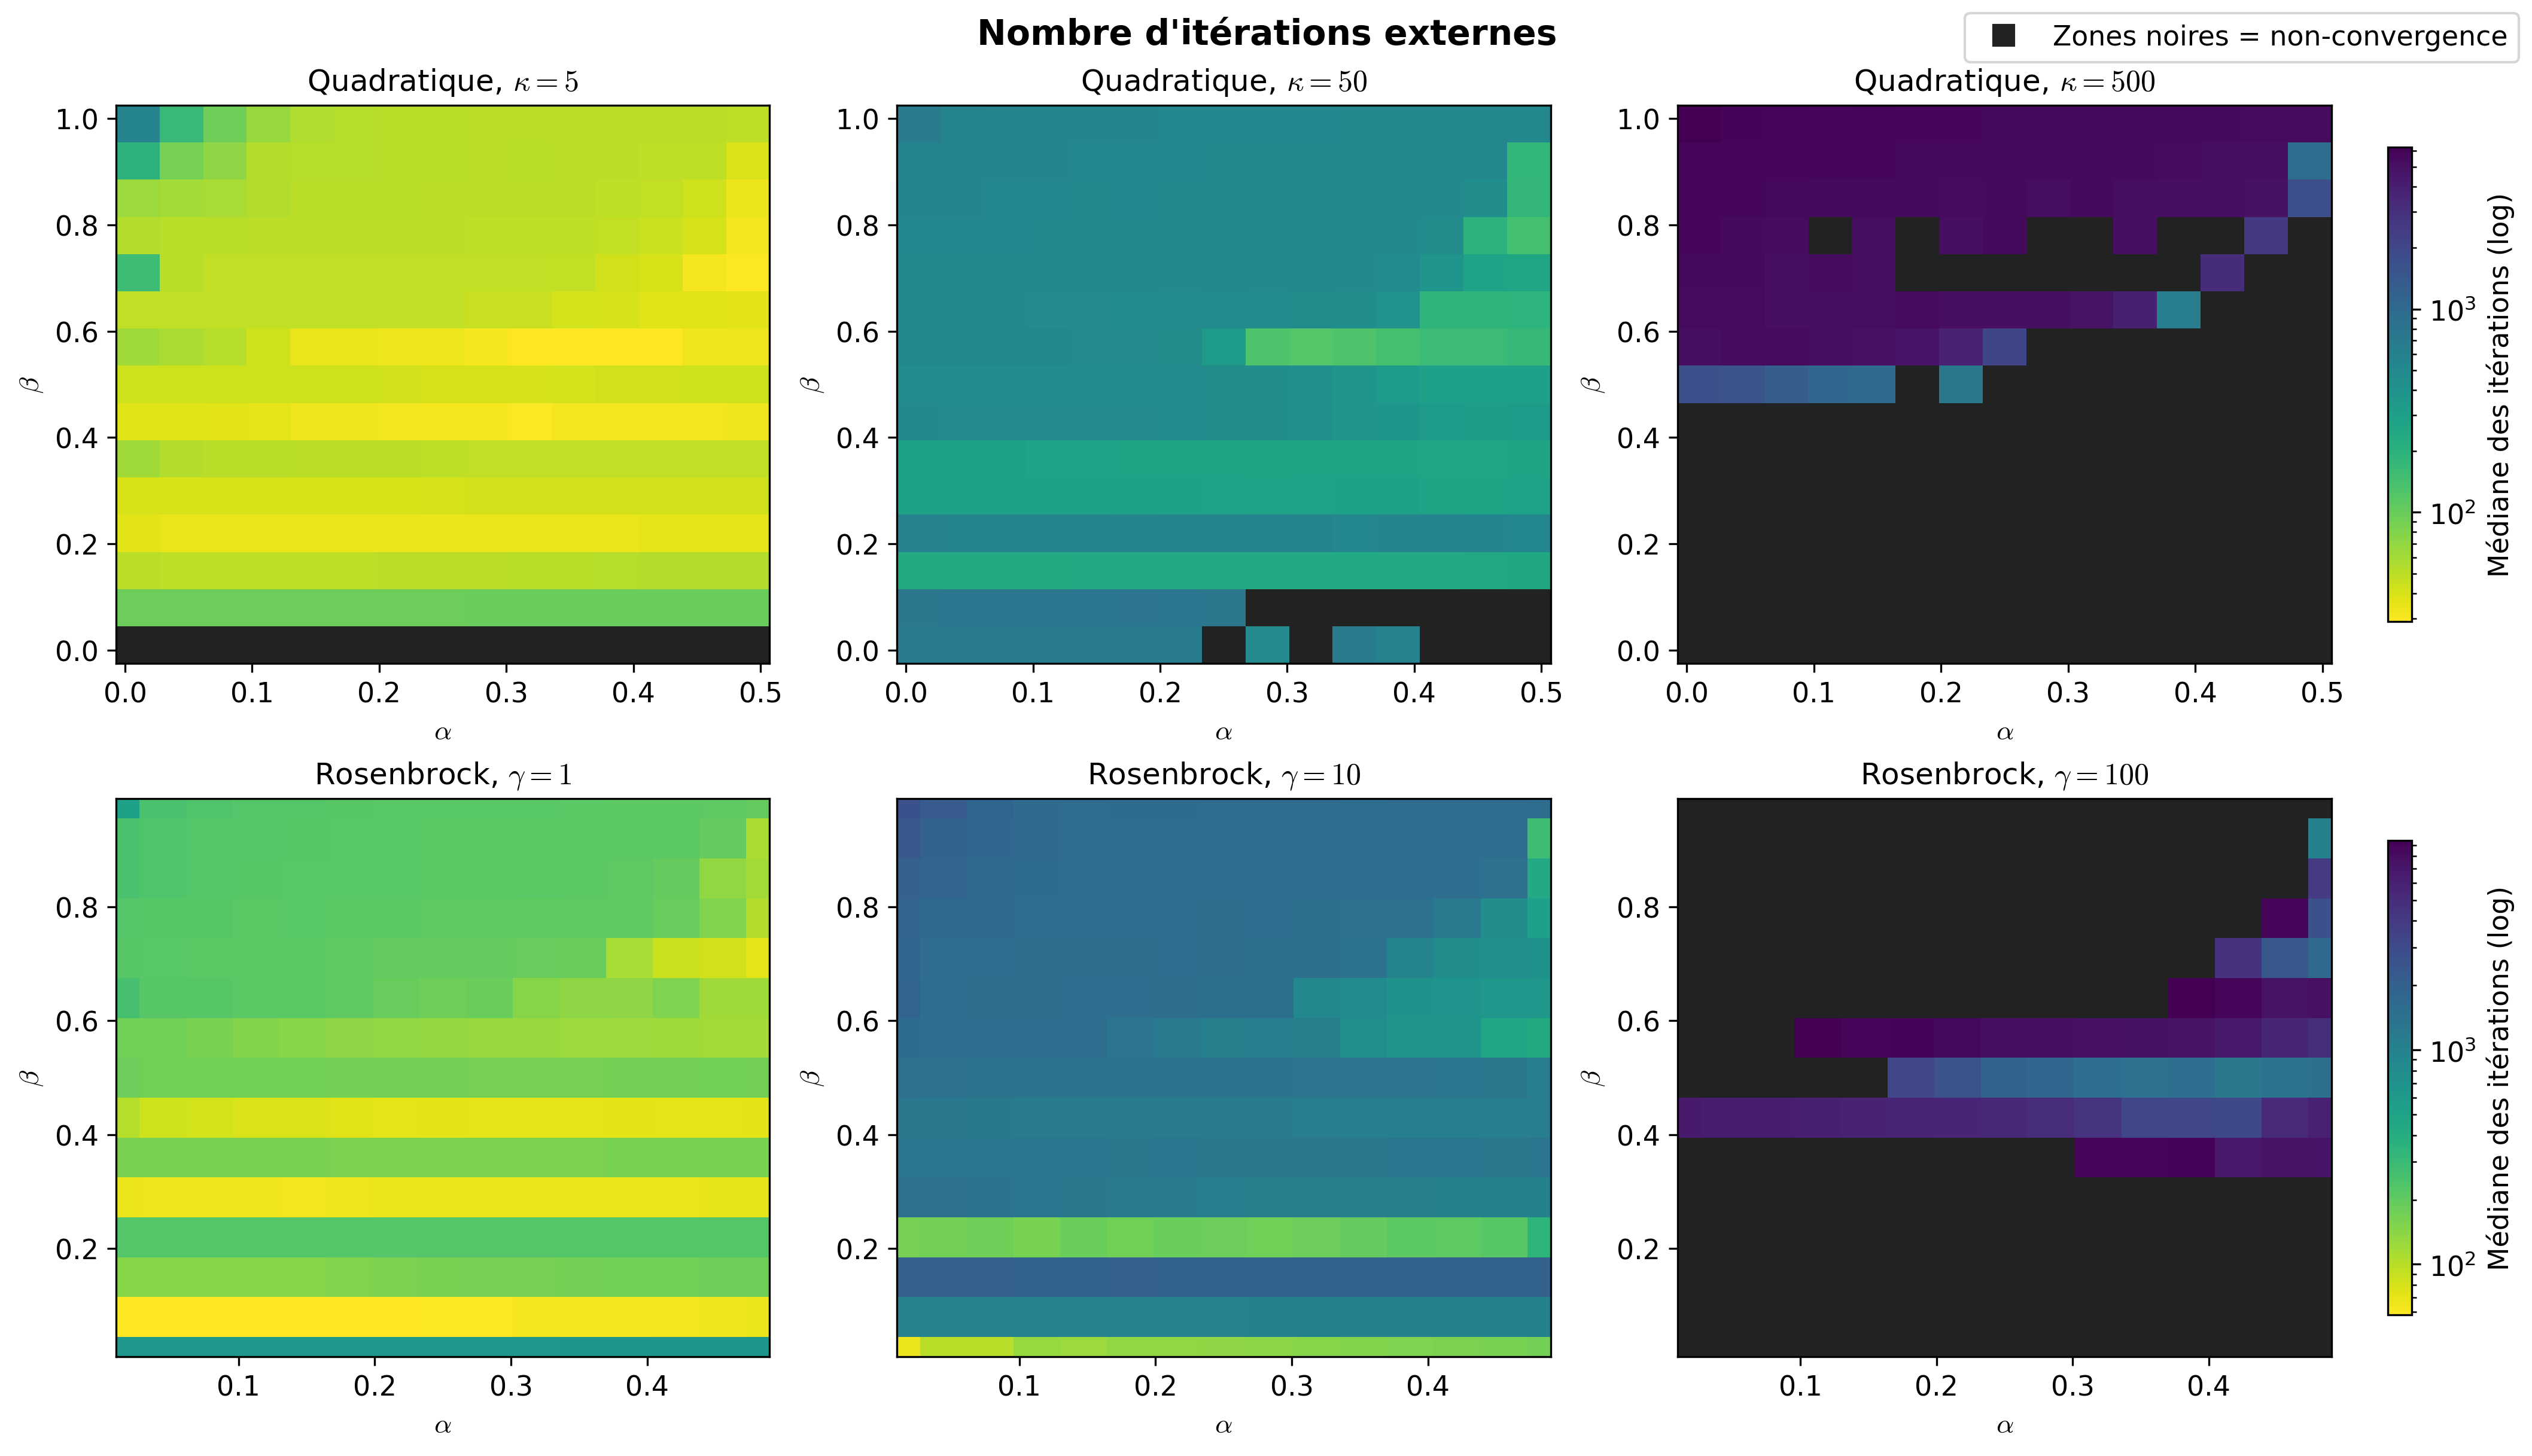
\includegraphics[width=\linewidth]{figures/benchmark1/graphique_1.png}
  \caption{Médiane du nombre d'itérations externes sur la grille $(\alpha,\beta)$. Ligne du haut~: $f_Q$ pour $\kappa \in \{5, 50, 500\}$~; ligne du bas~: $f_R$ pour $\gamma \in \{1, 10, 100\}$. Échelle de couleur logarithmique~; les zones noires indiquent un taux de convergence inférieur à $50\,\%$.}
  \label{fig:b1_iter}
\end{figure}

Pour $\beta$ proche de zéro, la boucle d'Armijo divise $\eta$ si brutalement que le pas effectif tombe sous la précision machine et l'algorithme stagne. Pour $\beta$ proche de un, la recherche linéaire finit par trouver un pas valide, mais au prix d'un nombre considérable d'évaluations de $f$ par itération~; à $\kappa = 50$ et $\beta = 0.99$, on relève en médiane environ 330 appels à $f$ par itération.

\begin{figure}[htbp]
  \centering
  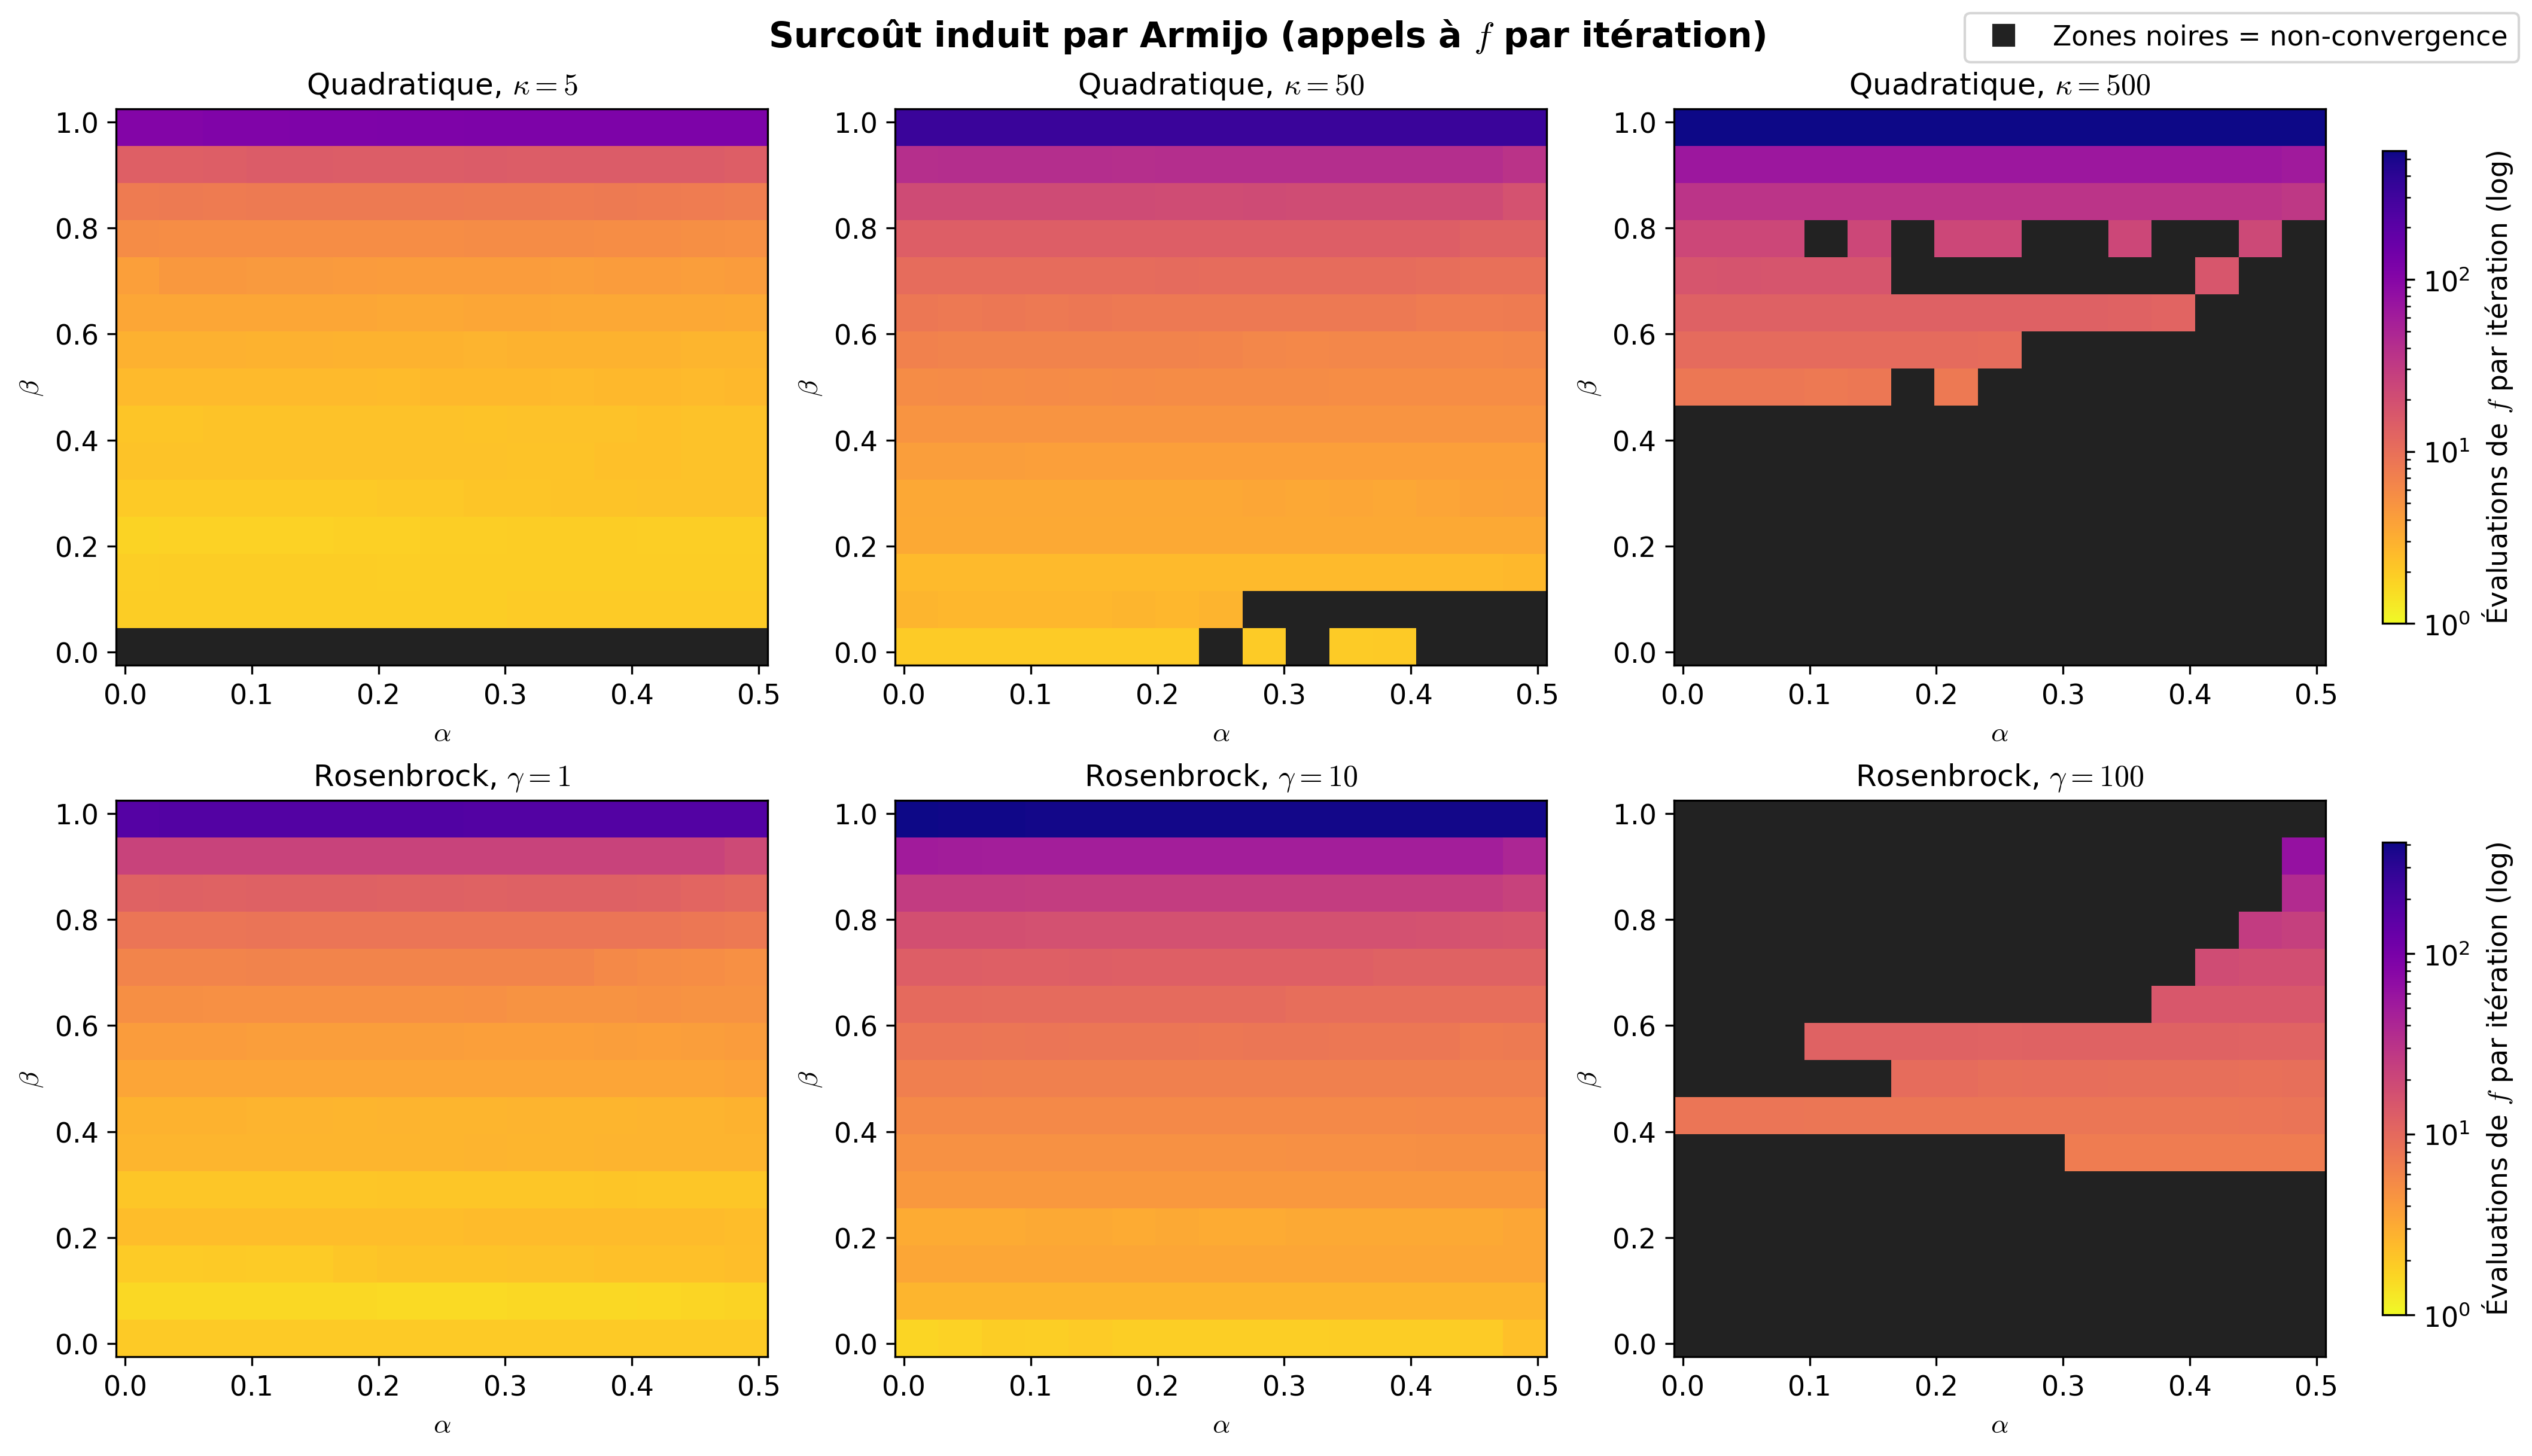
\includegraphics[width=\linewidth]{figures/benchmark1/graphique_2.png}
  \caption{Ratio du nombre d'évaluations de $f$ par itération (surcoût de la recherche d'Armijo). Ligne du haut~: $f_Q$ pour $\kappa \in \{5, 50, 500\}$~; ligne du bas~: $f_R$ pour $\gamma \in \{1, 10, 100\}$. Échelle de couleur logarithmique~; les zones noires indiquent un taux de convergence inférieur à $50\,\%$.}
  \label{fig:b1_fevals}
\end{figure}

Le conditionnement détermine la largeur de la zone convergente. À $\kappa = 5$, la quasi-totalité de la grille converge (taux de $94.5\%$, médiane d'environ 50 itérations)~; $\alpha$ et $\beta$ n'y jouent qu'un rôle marginal. À $\kappa = 500$, le taux s'effondre à $38\%$ et la bande convergente se réduit à $\beta \in [0.5, 0.99]$~: la borne en $O(\kappa \log(1/\varepsilon))$ prévoit une croissance linéaire du nombre d'itérations avec le conditionnement, et le plafond de $10^4$ itérations devient insuffisant pour une fraction croissante de la grille. La fonction de Rosenbrock confirme cette tendance~: la médiane d'itérations passe de 175 à $\gamma = 1$ à 1289 à $\gamma = 10$, puis à environ 5700 à $\gamma = 100$, soit un facteur d'environ 7 entre $\gamma = 1$ et $\gamma = 10$, et de 4 à 5 entre $\gamma = 10$ et $\gamma = 100$. À $\gamma = 100$, seulement $25\%$ des cellules convergent, dans une bande étroite autour de $\beta \in [0.4, 0.6]$ avec un $\alpha$ relativement élevé.

Le rôle de $\alpha$ se révèle précisément sur les régimes difficiles que l'on vient d'identifier, à savoir le grand $\kappa$ sur la fonction quadratique et le grand $\gamma$ sur la fonction de Rosenbrock, et de manière opposée selon la fonction. En régime bien conditionné, les cartes de chaleur sont quasiment horizontales~: $\alpha$ influence peu le résultat dès lors que $\beta$ est convenablement choisi (taux de convergence $\geq 93\%$ à $\kappa = 5$ pour tout $\alpha$, et $100\%$ à $\gamma = 1$).

Sur la fonction de Rosenbrock à $\gamma = 100$, le taux de convergence \emph{croît} nettement avec $\alpha$, passant de $4.9\%$ en moyenne à $\alpha = 0.01$ à $61.8\%$ à $\alpha = 0.49$. La vallée parabolique étroite engendre localement des directions où la valeur propre dominante de la hessienne est très grande, et il faut un $\alpha$ suffisamment proche de $1/2$ pour que la boucle d'Armijo rejette systématiquement le pas initial $\eta = 1$ et atterrisse dans la zone dynamiquement stable. La condition du critère d'Armijo joue alors le rôle d'un filtre de stabilité contre le dépassement.

Sur la fonction quadratique mal conditionnée, la situation s'inverse. À $\kappa = 500$, le taux de convergence \emph{décroît} avec $\alpha$, de $48.9\%$ à $\alpha = 0.01$ jusqu'à $23.6\%$ à $\alpha = 0.49$. Le ratio évaluations de $f$ par itération ne dépend que faiblement de $\alpha$ à $\beta$ fixé (médiane stable autour de $8.5$ à $\beta = 0.5$). Ce que $\alpha$ contrôle, c'est l'efficacité par itération parmi les instances qui aboutissent~: à $\beta = 0.5$, la médiane d'itérations chute de 1696 à 737 entre les deux extrêmes d'$\alpha$. Un $\alpha$ élevé sélectionne des pas plus exigeants en décroissance, mais rend la trajectoire plus sensible aux écarts par rapport au modèle quadratique idéal, ce qui fait échouer une fraction non négligeable des instances. La condition du critère d'Armijo joue ici un rôle de sélecteur de pas optimal plutôt que de filtre de stabilité.

\paragraph{Coût computationnel et compromis itérations / évaluations.}
À supposer que la convergence soit acquise, deux métriques quantifient le coût d'un réglage~: le nombre d'itérations externes et le nombre total d'évaluations de $f$. Si l'on note $n_k^{\text{Armijo}}$ le nombre de réductions du pas à l'itération $k$, le total d'évaluations s'écrit
\[
  \text{f-evals} \;=\; \sum_k \left(1 + n_k^{\text{Armijo}}\right),
\]
de sorte qu'un $\beta$ proche de $1$ produit un pas presque optimal à chaque itération au prix d'un $n_k^{\text{Armijo}}$ élevé, là où un $\beta$ plus faible termine la boucle d'Armijo en quelques étapes mais avec un pas conservateur qui rallonge le nombre d'itérations. La figure~\ref{fig:b1_pareto} reporte chaque cellule $(\alpha, \beta)$ dans le plan (itérations, évaluations) et fait apparaître le front de Pareto correspondant. Dans les régimes faciles à intermédiaires ($\kappa \in \{5, 50\}$, $\gamma \in \{1, 10\}$), ce front se situe à $\beta$ petit (entre $0.01$ et $0.57$ selon le régime)~: le coût d'une recherche linéaire courte est négligeable et il vaut mieux économiser les évaluations. Dans les régimes sévères ($\kappa = 500$, $\gamma = 100$), le front se déplace vers $\beta \approx 0.5$, l'étroite marge de progression par itération imposant alors un pas presque optimal.

\begin{figure}[htbp]
  \centering
  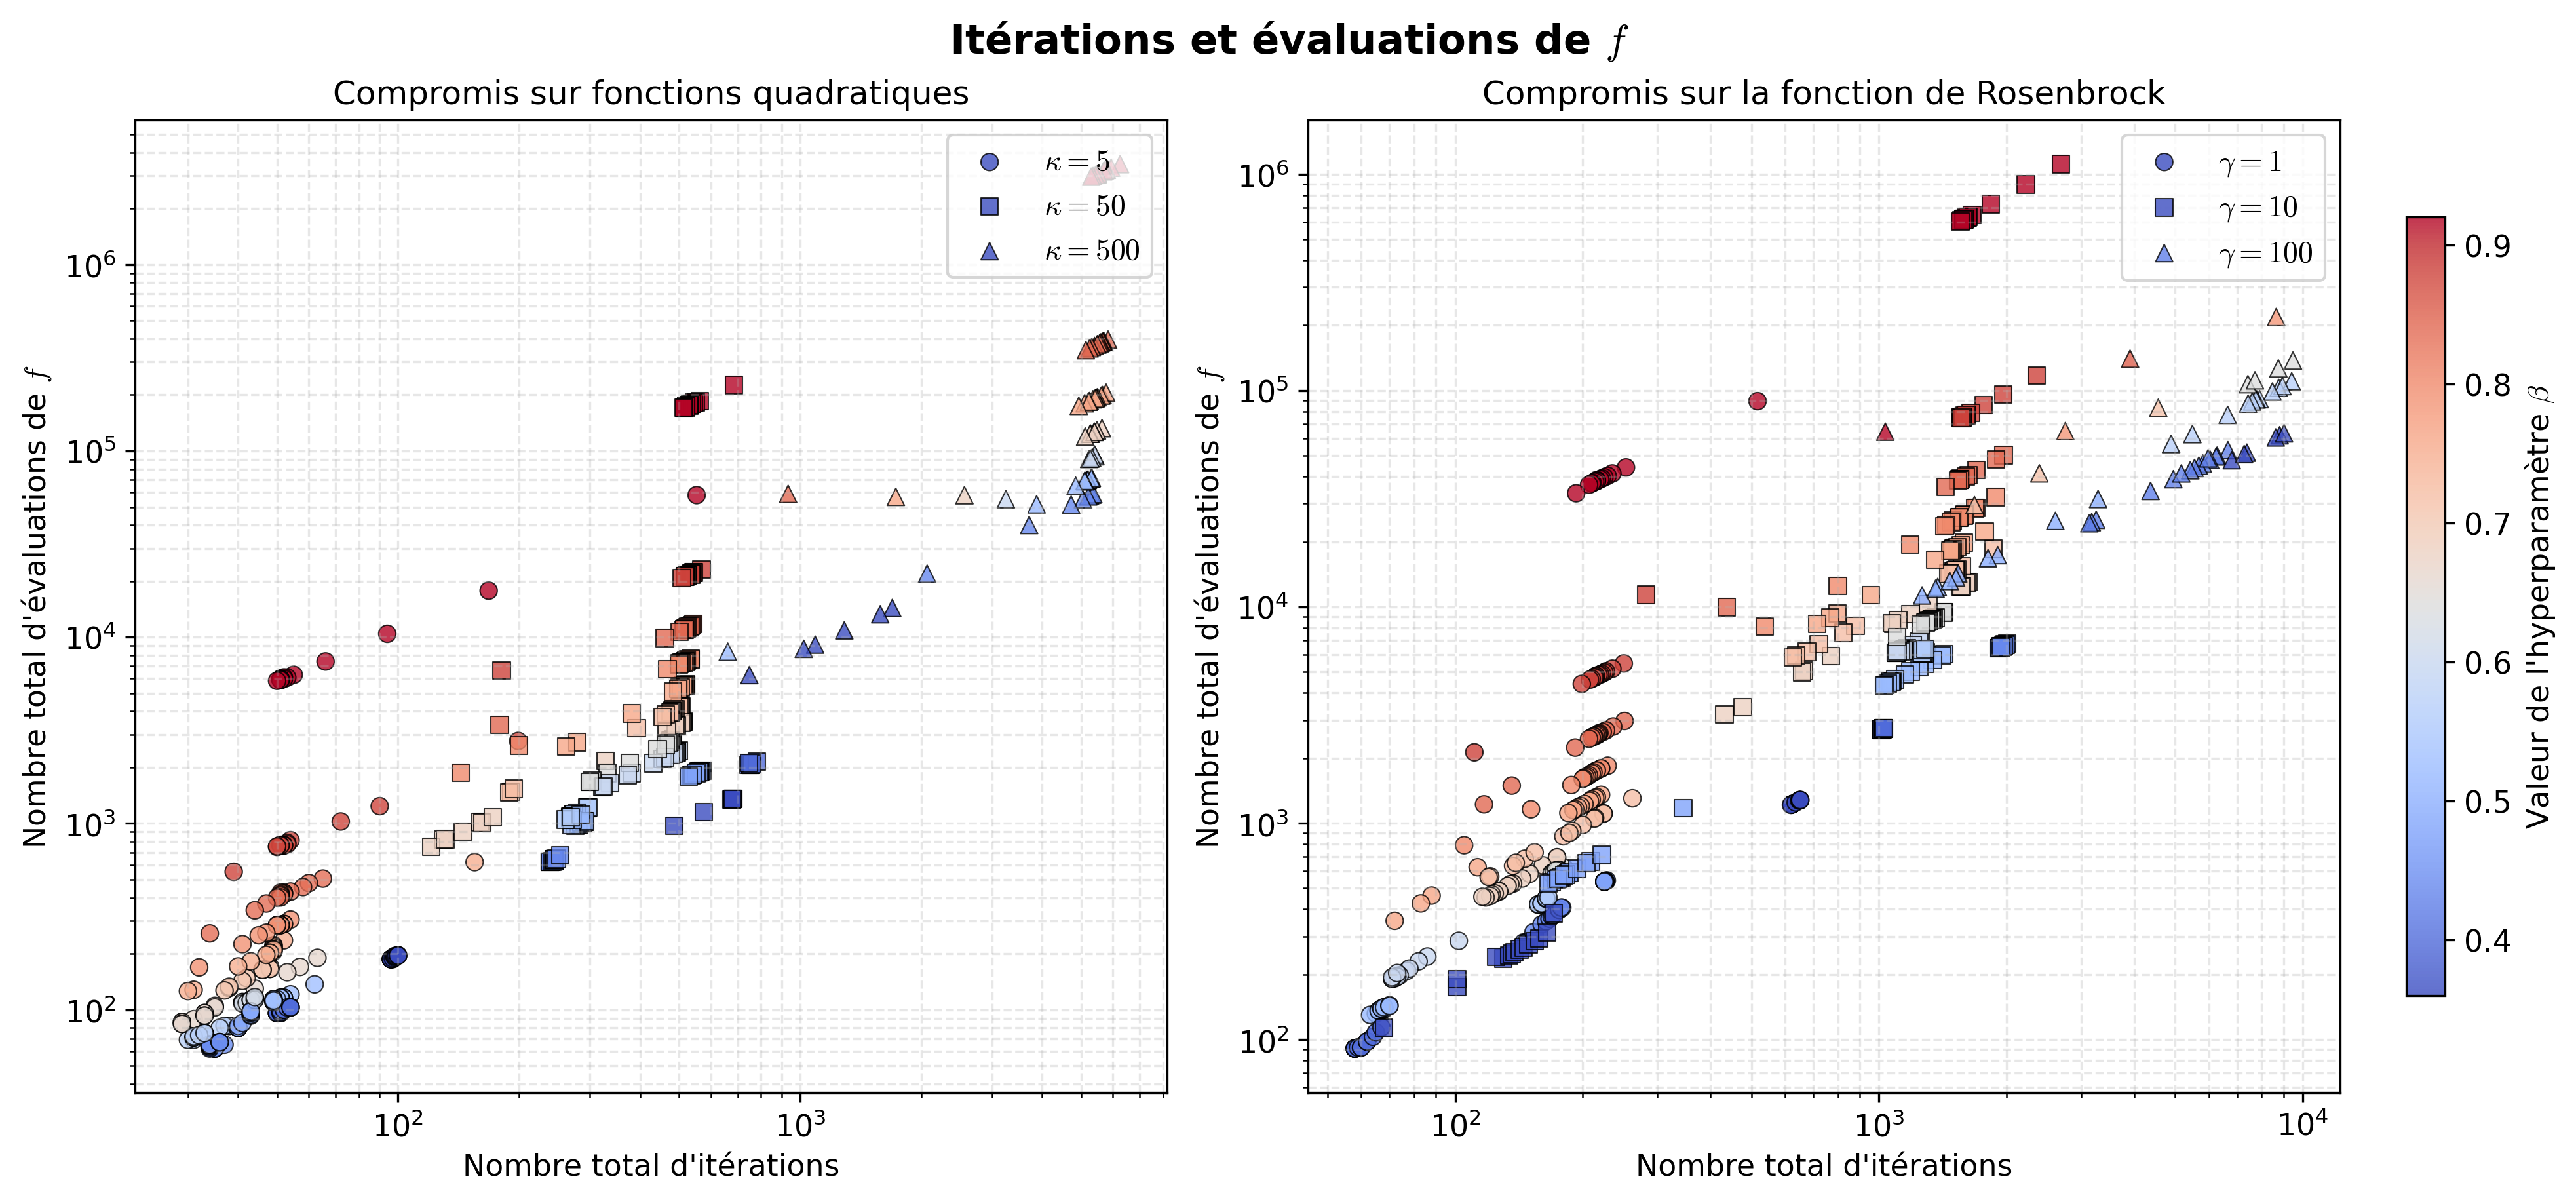
\includegraphics[width=\linewidth]{figures/benchmark1/graphique_3.png}
  \caption{Compromis entre itérations et évaluations de $f$ sur la grille $(\alpha,\beta)$, en échelle log-log. Gauche~: $f_Q$ ($\kappa \in \{5, 50, 500\}$, distingués par forme de marqueur)~; droite~: $f_R$ ($\gamma \in \{1, 10, 100\}$). La couleur code la valeur de $\beta$ (bleu~: $\beta$ faible~; rouge~: $\beta$ élevé).}
  \label{fig:b1_pareto}
\end{figure}

Le cas $\kappa = 500$ met en évidence une dissociation~: la valeur de $\beta$ qui maximise le taux de convergence n'est pas celle qui minimise le coût opérationnel. Entre $\beta = 0.5$ (taux de $49\%$) et $\beta = 0.99$ (taux de $72\%$), la médiane d'évaluations de $f$ croît d'environ deux ordres et demi de grandeur. On échange ainsi ce surcoût contre vingt-trois points de pourcentage de fiabilité. Si l'objectif est de minimiser la probabilité d'échec d'une exécution unique, un $\beta$ proche de $1$ est le choix indiqué~; si l'objectif est le débit computationnel global, $\beta \approx 0.5$ reste préférable, le surcoût d'un éventuel nouveau tirage étant largement absorbé par l'écart de coût unitaire.

\paragraph{Dynamique de convergence et confrontation à la borne théorique.}
Lorsqu'elles atteignent leur régime asymptotique, les trajectoires présentent une contraction géométrique compatible avec la borne $\rho^k$~; aux conditionnements élevés, ce régime n'est pas toujours atteint dans le budget de $10^4$ itérations, comme le confirme le tableau~\ref{tab:rho}. La figure~\ref{fig:b1_traj} reporte $\|x_k - x^\star\|_2$ pour quatre paires représentatives~: $\beta$ faible $(0.04,\,0.22)$, Boyd $(0.25,\,0.50)$, $\beta$ modéré $(0.10,\,0.70)$ et $\beta$ élevé $(0.10,\,0.92)$.

\begin{figure}[htbp]
  \centering
  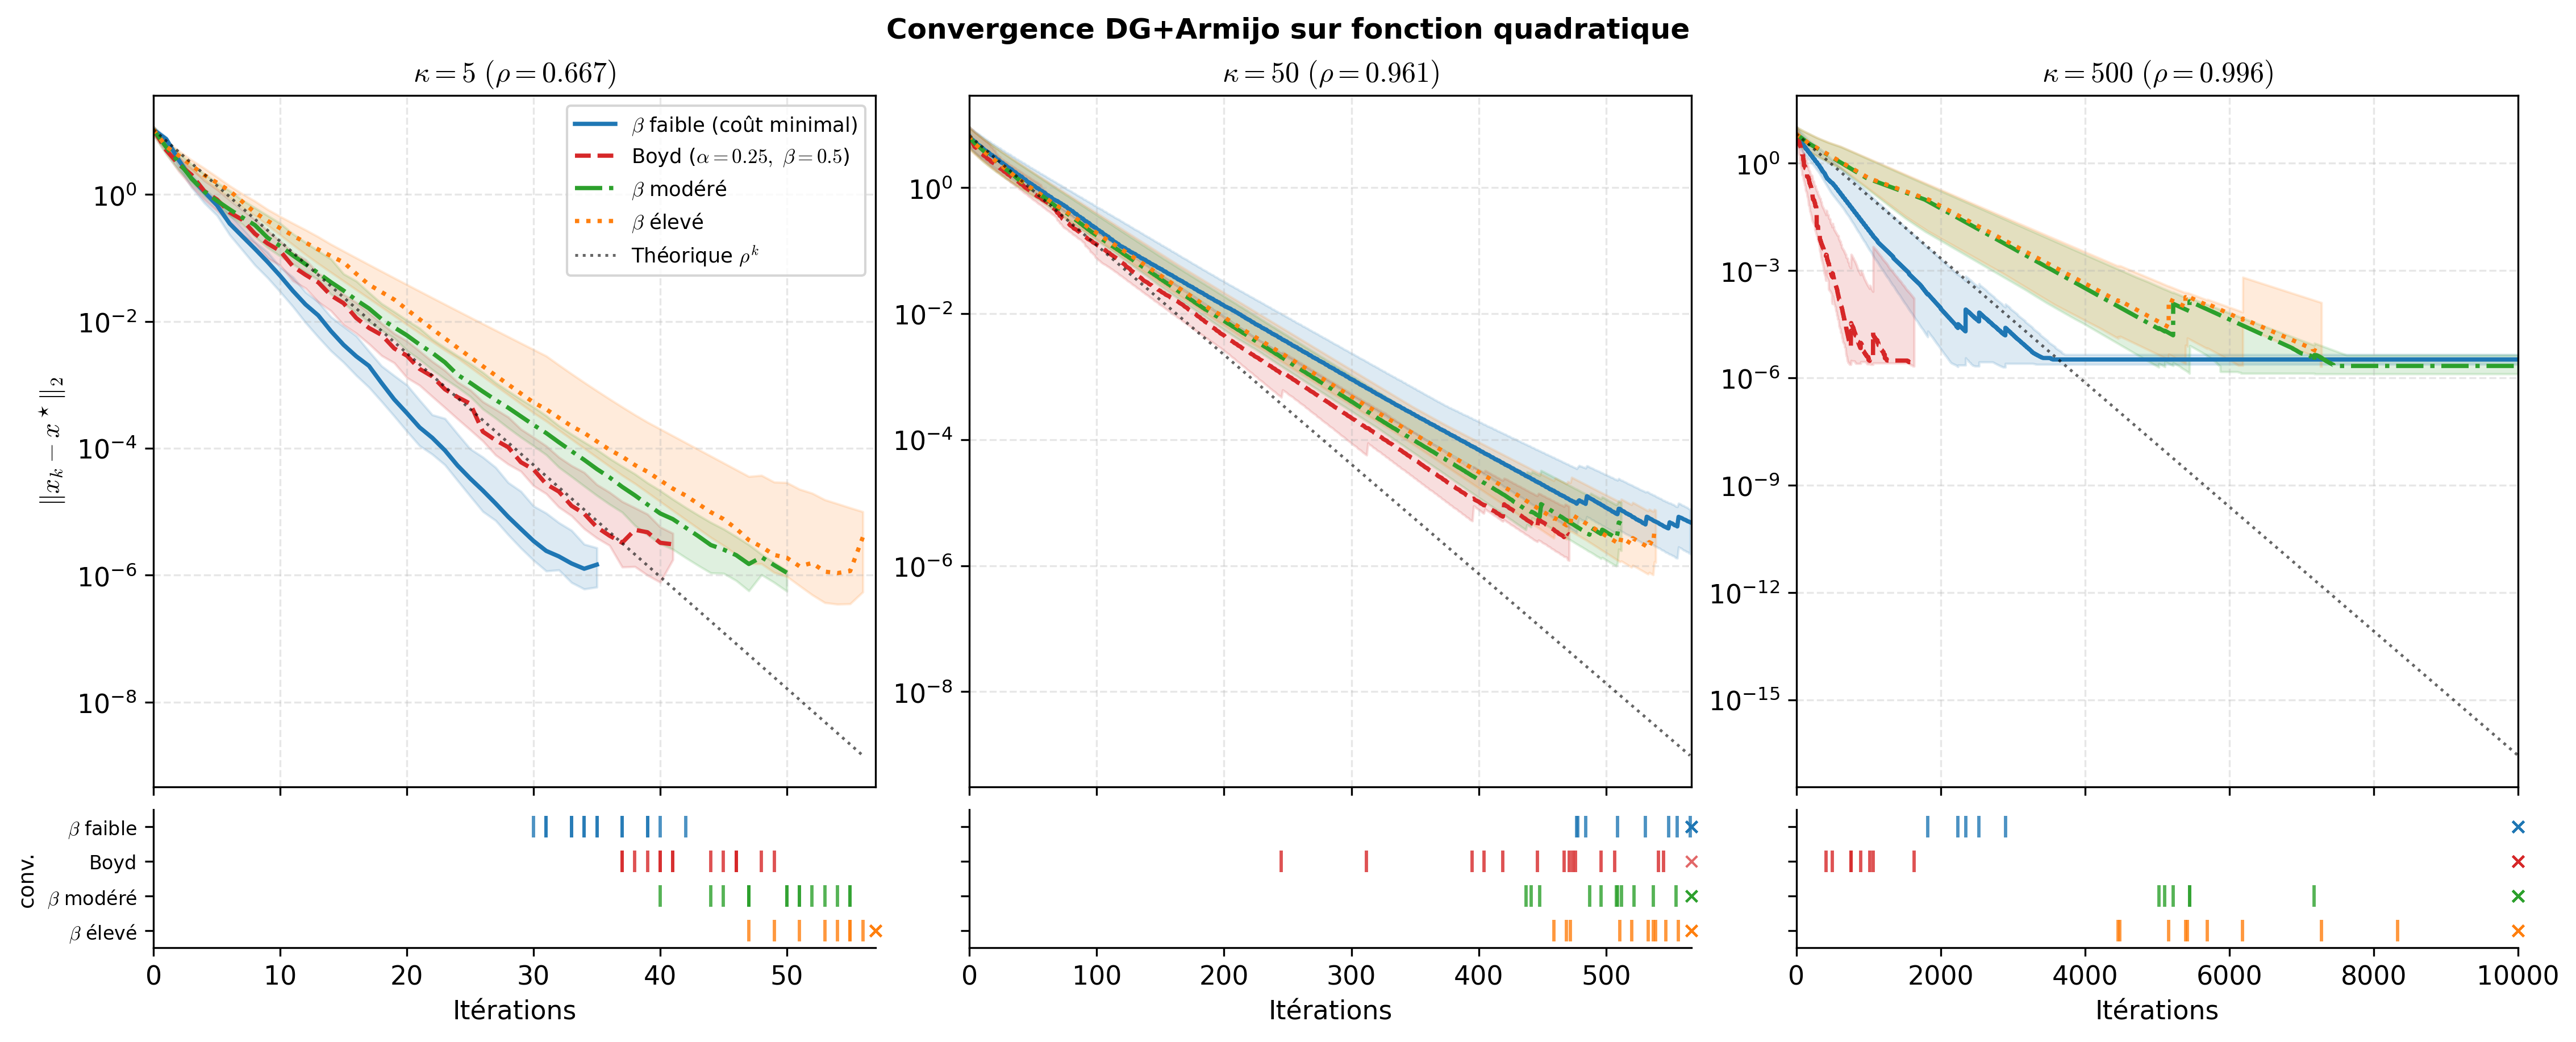
\includegraphics[width=\linewidth]{figures/benchmark1/graphique_4.png}
  \caption{Convergence de la descente de gradient avec critère d'Armijo sur $f_Q$ pour quatre paires $(\alpha,\beta)$~: $\|x_k - x^\star\|_2$ en fonction de $k$, médiane $\pm$ IQR sur 15 instances. De gauche à droite~: $\kappa \in \{5, 50, 500\}$. Pointillés gris~: borne théorique $\rho^k \|x_0-x^\star\|_2$. La bande inférieure indique, pour chaque paire, l'itération de convergence par instance (\texttt{|}) ou le report au bord droit en cas de non-convergence dans la fenêtre représentée (\texttt{$\times$}).}
  \label{fig:b1_traj}
\end{figure}

À $\kappa = 5$, les quatre paires convergent rapidement, en un peu moins de soixante itérations en médiane. Les écarts entre paires sont visibles mais modestes : la paire à $\beta$ faible $(\alpha = 0.04, \beta = 0.22)$ atteint le critère avec une médiane de 35 itérations, contre 56 pour la paire à $\beta$ élevé $(\alpha = 0.10, \beta = 0.92)$. Les marqueurs révèlent une dispersion inter-instances très faible (ratio max/min compris entre 1.3 et 1.6 selon la paire)~: à ce conditionnement, le compteur d'itérations est essentiellement déterministe, l'instance n'introduit qu'une variabilité de second ordre.

À $\kappa = 50$, l'ordre des paires s'inverse et leurs trajectoires se rapprochent~: les médianes vont de 471 (Boyd) à 556 ($\beta$ faible), soit un écart relatif inférieur à $20\%$. Cette homogénéité cache toutefois une asymétrie de dispersion~: Boyd s'étale de 245 à 603 itérations (ratio 2.5), tandis que les trois autres paires conservent un ratio max/min inférieur à 1.5. Le réglage le plus rapide en médiane est aussi celui dont les performances dépendent le plus de l'instance.

C'est à $\kappa = 500$ que le comportement se transforme qualitativement. La convergence devient partielle~: $\beta$ faible converge sur 5 instances sur 15, Boyd sur 7, $\beta$ modéré sur 6 et $\beta$ élevé sur 9. Boyd reste le plus rapide en médiane (824 itérations) mais converge sur moins d'instances que $\beta$ élevé (médiane 5417)~: le compromis fiabilité-vitesse, invisible aux conditionnements plus faibles, s'impose à $\kappa$ sévère et oppose deux régimes désormais distincts.

La pente effective de chaque trajectoire peut être confrontée à la borne théorique. Pour chaque paire et chaque conditionnement, on extrait par régression linéaire de $\log \|x_k - x^\star\|_2$ sur la zone d'allure géométrique (typiquement $k$ compris entre 20 et $k_{\text{fin}} - 5$) un taux de contraction empirique $\rho_{\text{emp}}$. Le tableau~\ref{tab:rho} reporte ces valeurs en regard de la borne $\rho_{\text{theo}} = (\kappa - 1) / (\kappa + 1)$.

\begin{table}[htbp]
\centering
\small
\begin{tabular}{l|cccc|c}
\toprule
 & $\beta$ faible & Boyd & $\beta$ modéré & $\beta$ élevé & $\rho_{\text{theo}}$ \\
\midrule
$\kappa = 5$   & 0.652 & 0.707 & 0.734 & 0.786 & 0.667 \\
$\kappa = 50$  & 1.000 & 0.975 & 0.976 & 0.976 & 0.961 \\
$\kappa = 500$ & 0.999 & 1.000 & 0.999 & 0.999 & 0.996 \\
\bottomrule
\end{tabular}
\caption{Taux de contraction empirique $\rho_{\text{emp}}$ par paire, confronté à la borne théorique $\rho_{\text{theo}}$. Une valeur $\rho_{\text{emp}} = 1.000$ signifie que la trajectoire n'a pas atteint le régime géométrique dans les $10^4$ itérations allouées.}
\label{tab:rho}
\end{table}

Le résultat se lit en trois temps. À $\kappa = 5$, les valeurs empiriques se situent légèrement au-dessus de la borne pour trois paires sur quatre, traduisant le surcoût que le critère d'Armijo paie par rapport au pas optimal. Pour la paire à $\beta$ faible, $\rho_{\text{emp}} = 0.652 < \rho_{\text{theo}} = 0.667$~: la borne majore le pire cas et n'est pas atteinte en général. À $\kappa = 50$, l'accord est bon ($\rho_{\text{emp}}$ entre $0.975$ et $0.976$ contre $\rho_{\text{theo}} = 0.961$)~; la paire à $\beta$ faible affiche $\rho_{\text{emp}} \approx 1$, signe qu'elle n'atteint pas son régime géométrique dans le budget alloué. À $\kappa = 500$, toutes les paires affichent $\rho_{\text{emp}} \approx 1$, même phénomène à plus grande échelle. La borne théorique reste un bon indicateur de la pente effective, à condition que la trajectoire soit observée sur sa zone géométrique.

\paragraph{Cas non-convexe~: trajectoires sur la fonction de Rosenbrock.}
La figure~\ref{fig:b1_traj_rosen} reporte les mêmes quatre paires sur la fonction de Rosenbrock à $\gamma \in \{1, 10, 100\}$. La borne en $\rho^k$ n'admet plus d'équivalent global, mais la comparaison directe des trajectoires fait apparaître trois régimes qualitativement distincts qui complètent l'analyse quadratique.

\begin{figure}[htbp]
  \centering
  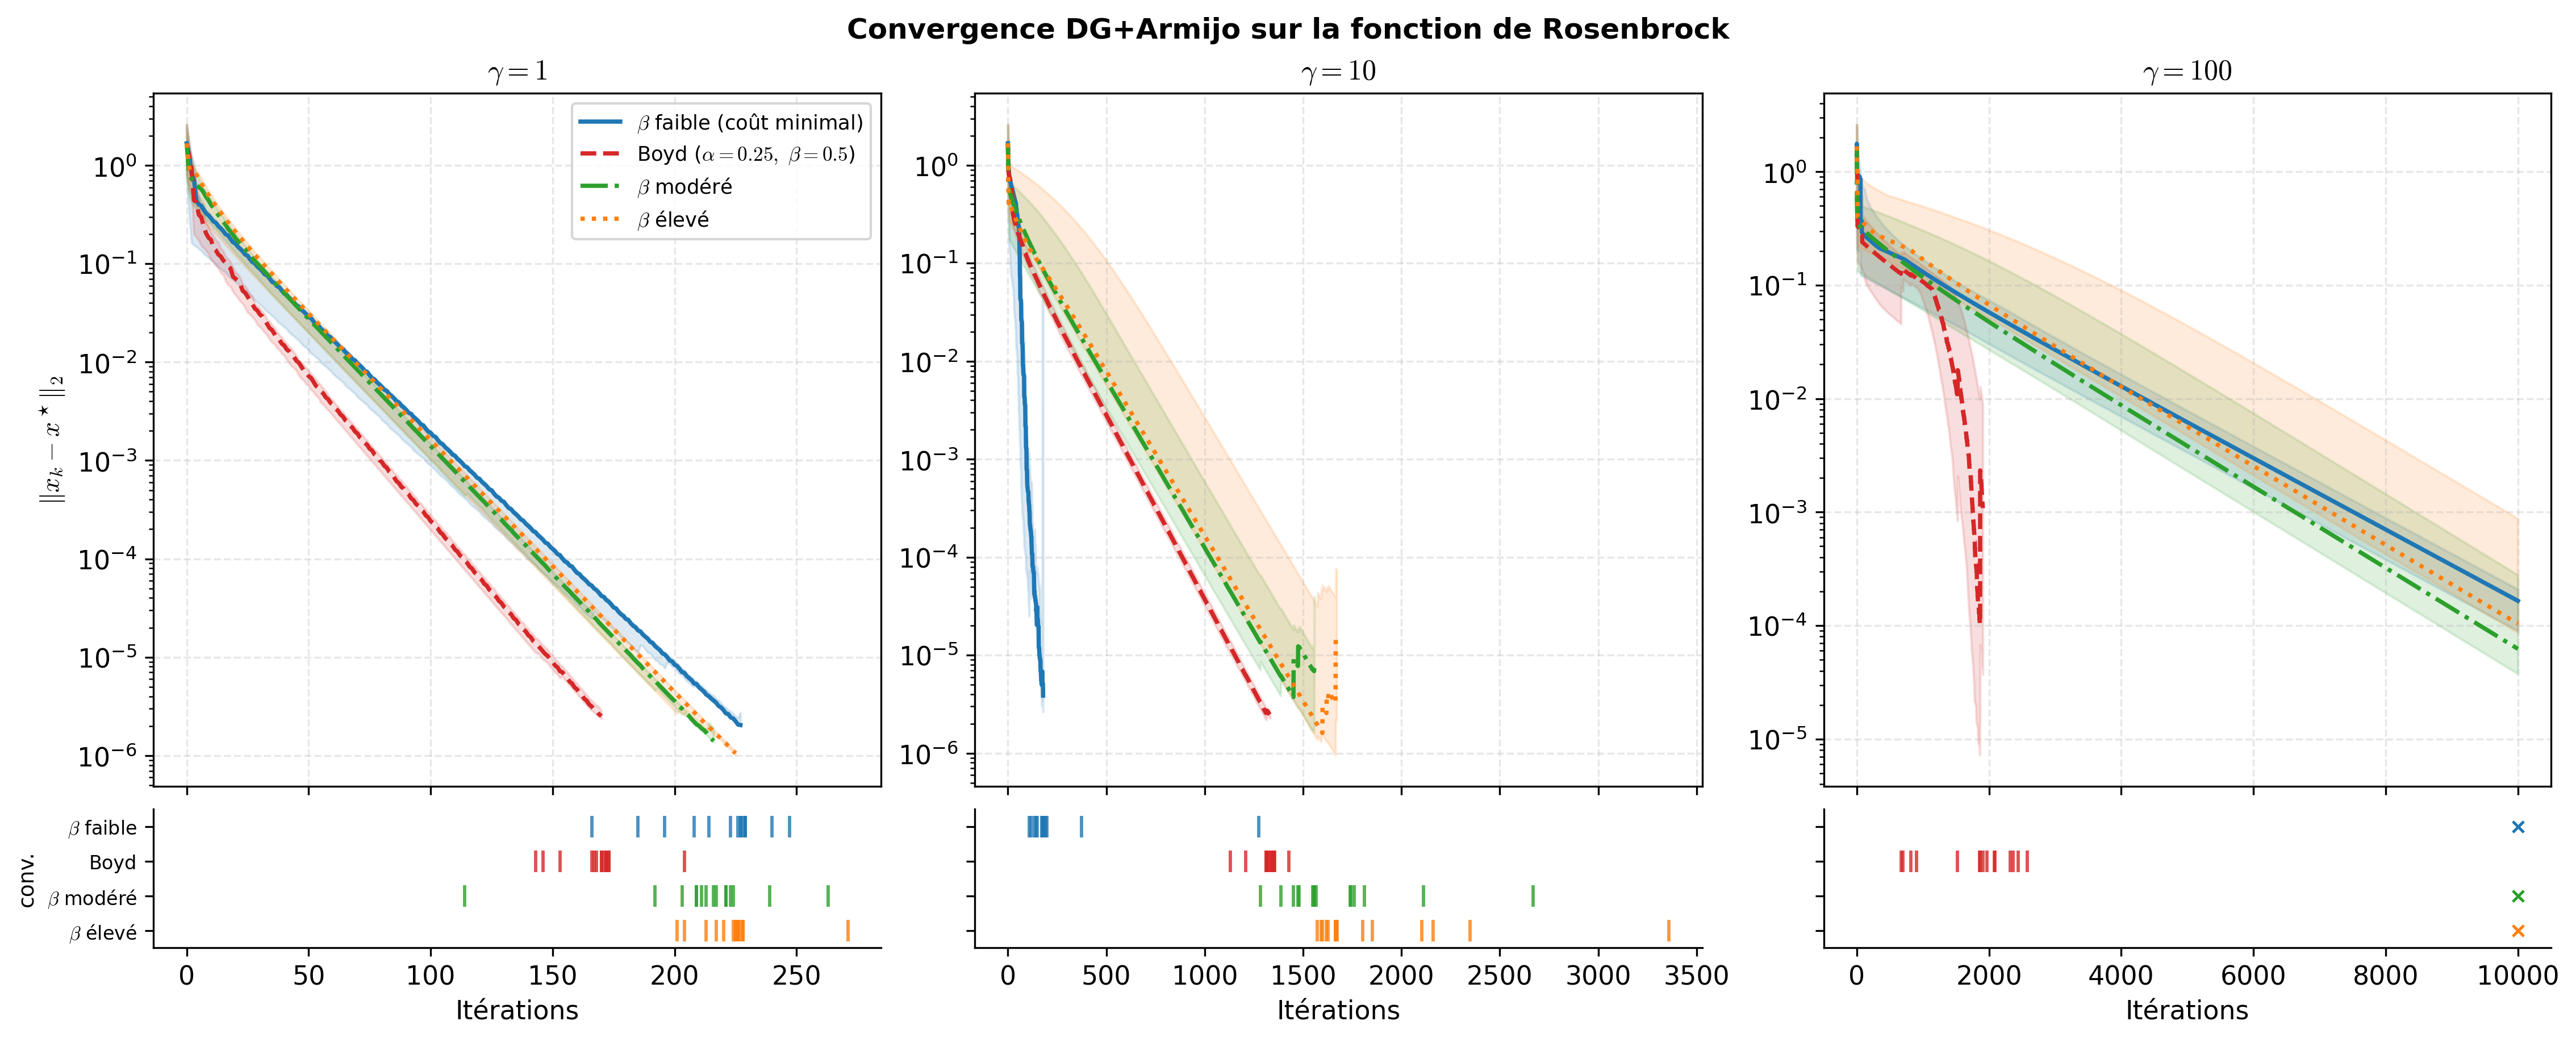
\includegraphics[width=\linewidth]{figures/benchmark1/graphique_5.png}
  \caption{Convergence de la descente de gradient avec critère d'Armijo sur $f_R$ pour les quatre mêmes paires $(\alpha, \beta)$~: $\|x_k - x^\star\|_2$ en fonction de $k$, médiane $\pm$ IQR sur 15 points initiaux. De gauche à droite~: $\gamma \in \{1, 10, 100\}$. Bande inférieure~: itération de convergence par instance (\texttt{|}) ou report au bord droit en cas de non-convergence dans $10^4$ itérations (\texttt{$\times$}).}
  \label{fig:b1_traj_rosen}
\end{figure}

À $\gamma = 1$, les quatre paires convergent pour les 15 instances avec des médianes de 170 à 227 itérations. L'allure semi-logarithmique reste quasi-linéaire~: la non-linéarité de $f_R$ est suffisamment faible pour que le comportement local quadratique domine, et la dispersion inter-instances reste du même ordre que celle du cas $\kappa = 5$.

À $\gamma = 10$, la dynamique se réorganise de façon inattendue. La paire $\beta$ faible converge avec une médiane de 179 itérations contre 1332 pour Boyd, soit un rapport de 7.4, exactement l'ordre inverse du cas quadratique. Un $\alpha$ proche de zéro relâche l'exigence de décroissance suffisante~: la boucle d'Armijo termine, en moyenne, en 3.2 évaluations de $f$ par itération pour $\beta$ faible contre 6.6 pour Boyd, ce qui produit un pas effectif sensiblement plus grand. La géométrie de $f_R$ à $\gamma = 10$ tolère encore ces grands pas sans déclencher d'instabilité. Les marqueurs révèlent néanmoins le revers~: une instance isolée pour $\beta$ faible converge en 1274 itérations contre une médiane de 179, tandis que les trois autres paires restent sous une moyenne de 2.2. La paire $\beta$ faible est donc rapide en moyenne mais comporte un risque de queue de distribution que la seule médiane ne suffit pas à exposer.

À $\gamma = 100$, le comportement devient binaire. Seul le réglage de Boyd converge, et il le fait pour les 15 instances (médiane 1907 itérations, écart 669 à 2583)~; les trois autres paires plafonnent à $10^4$ itérations sur l'intégralité des instances. Les marqueurs rendent cette dichotomie immédiatement visible avec, pour chaque paire défaillante, 15 croix alignées au bord droit. La trajectoire médiane de Boyd présente une structure en trois phases que n'admet aucune trajectoire quadratique. D'abord un transitoire rapide~: l'erreur passe de $\|x_0 - x^\star\| \approx 1.7$ à $\approx 0.3$ en une quinzaine d'itérations, le long du gradient en dehors de la vallée. Suit une longue progression sous-linéaire à l'intérieur de la vallée parabolique (un facteur 2.5 sur 600 itérations). Enfin, une queue quasi-linéaire dans le régime localement quadratique au voisinage de $(1,1)$. Aucun taux de contraction unique ne décrit l'ensemble de la trajectoire, là où le cas quadratique reste géométrique d'un bout à l'autre.

\paragraph{Synthèse opérationnelle.}
Boyd n'est pas Pareto-optimal en régime facile, le front s'y situe à des $\beta$ bien plus petits (approximativement $0.22$ à $\kappa = 5$, $0.15$ à $\kappa = 50$), mais c'est le seul réglage universellement convergent~: $100\%$ partout sauf à $\kappa = 500$ ($47\%$), là où les trois autres paires échouent uniformément à $\gamma = 100$. Lorsque le conditionnement est connu et modeste, abaisser $\beta$ vers le front de Pareto réduit le coût~; la remontée à $\kappa$ sévère reflète le besoin d'une recherche linéaire fine quand la marge par itération devient étroite. En régime sévère, c'est sur $\alpha$ qu'il faut jouer~: pousser $\alpha$ vers $0.4$ filtre les pas instables et débloque la convergence dans des régions où aucun choix de $\beta$ ne suffit. L'analyse instance par instance confirme ce constat~: à $\gamma = 100$, Boyd converge sur l'intégralité des 15 instances. La condition du critère d'Armijo change ainsi de rôle selon la géométrie~: filtre de stabilité sur la vallée de Rosenbrock, sélecteur de pas optimal sur la fonction quadratique mal conditionnée. En l'absence d'information préalable, $\beta = 0.5$ reste un choix par défaut robuste.

\newpage

\subsection{Benchmark 2~: Fletcher-Reeves contre Polak-Ribière sur des fonctions non-convexes}\label{sec:b2}

\subsubsection{Protocole expérimental}

Ce benchmark étudie si, sur des fonctions non-convexes, les méthodes de gradient conjugué FR et PR convergent vers les mêmes minima locaux et avec la même robustesse. Les deux algorithmes ne diffèrent que par leur formule de $\beta_k$~; toute divergence de comportement est donc imputable à ce seul choix.

\paragraph{Fonctions test.} Trois des quatre familles introduites en section~\ref{sec:fonctions} sont étudiées, chacune paramétrée par $\gamma$ pour en contrôler la difficulté.

\begin{itemize}
    \item \textbf{Multitrous} $f_M$, avec $\gamma \in \{1, 2, 4, 8\}$. Le terme oscillant $\cos(x^2)$ engendre plusieurs puits locaux~; le terme quadratique en contrôle la profondeur relative. Le nombre de minima locaux accessibles décroît avec $\gamma$.
    \item \textbf{Cubique} $f_C$, avec $\gamma \in \{1, 5, 10\}$. À $\gamma = 1$, le discriminant de $f_C' = 0$ est négatif~: la fonction n'admet aucun point critique et diverge vers $-\infty$, fournissant un test de robustesse à la divergence. À $\gamma \in \{5, 10\}$, un minimum local apparaît, dont le bassin d'attraction croît avec $\gamma$.
    \item \textbf{Rosenbrock} $f_R$, avec $\gamma \in \{1, 10, 100\}$. Un seul minimum global~: les deux méthodes convergent toujours, mais la vitesse diffère.
\end{itemize}

\paragraph{Grille de points initiaux.} Pour chaque couple (fonction, $\gamma$), on construit une grille régulière $50 \times 50$ de points initiaux sur le domaine pertinent~: $[-4, 4]^2$ pour $f_M$, $[-4, 2]^2$ pour $f_C$, $[-2, 3]^2$ pour $f_R$, soit 2500 exécutions par configuration et par méthode. Cette couverture exhaustive du domaine est strictement plus forte qu'un tirage aléatoire de même taille~: elle garantit qu'aucune région n'est manquée par malchance d'échantillonnage.

\paragraph{Choix algorithmiques.} Les deux méthodes utilisent la même recherche linéaire d'Armijo avec $(\alpha, \beta) = (0.25, 0.5)$, le même critère d'arrêt $\|\nabla f(x_k)\| < 10^{-6}$ et la même limite de $10^4$ itérations. Aucun redémarrage explicite n'est appliqué lorsque la direction $d_k$ n'est plus une direction de descente ($\langle \nabla f(x_k), d_k \rangle \geq 0$). Ce choix est délibéré~: c'est précisément ce que le benchmark mesure. Sur des fonctions non-convexes, $\beta_k^{\text{PR}}$ peut devenir négatif, inversant la contribution de la direction précédente~; $\beta_k^{\text{FR}}$, toujours positif, accumule du moment dans la direction précédente même lorsque celle-ci est devenue inadaptée. Ajouter un redémarrage explicite aux deux méthodes pourrait atténuer cette différence structurelle. Un test de divergence ($|f(x_k)| > 10^8$ ou coordonnées non finies) interrompt les exécutions ayant quitté le domaine numérique utile, ce qui se produit principalement sur $f_C$ à $\gamma = 1$.

\paragraph{Vérification sur la fonction quadratique.} En préambule, on vérifie empiriquement l'équivalence théorique sur la fonction $f_Q$ en dimension 2 avec recherche linéaire exacte ($\eta_k = -\langle \nabla f_k, d_k\rangle / (d_k^\top A d_k)$) à deux conditionnements ($\kappa \in \{5, 50\}$). Sous cette hypothèse, les directions successives sont $A$-orthogonales (conjuguées) et les gradients successifs sont orthogonaux au sens euclidien, d'où $\langle \nabla f_k, \nabla f_{k-1}\rangle = 0$ et $\beta_k^{\text{PR}} = \beta_k^{\text{FR}}$. Les trajectoires et compteurs d'itérations doivent coïncider exactement.

\paragraph{Métriques.} Pour chaque exécution, on enregistre le nombre d'itérations, la valeur $f(x_{\text{final}})$, la position finale $(x_1, x_2)$ et un indicateur de convergence. La position finale est classée par proximité ($\ell_2 < 0.5$) au minimum global identifié par évaluation sur grille fine ($500 \times 500$) pour $f_M$, analytiquement pour $f_R$, et au minimum local (la fonction étant non bornée inférieurement) pour $f_C$.

\subsubsection{Résultats et Analyse}

L'analyse s'organise en cinq temps. On vérifie d'abord l'équivalence théorique sur la fonction quadratique. On caractérise ensuite les bassins d'attraction sur la fonction multitrous, puis sur la fonction cubique non bornée. On étudie alors la vitesse de convergence conditionnelle, c'est-à-dire le coût en itérations \emph{parmi les exécutions qui aboutissent}, avant de dégager une synthèse.

\paragraph{Équivalence sur la fonction quadratique.}
Les trajectoires FR et PR coïncident point par point dans les six configurations testées ($\kappa \in \{5,50\}$, trois points initiaux), comme le montre la figure~\ref{fig:b2_quad}. L'explication est immédiate~: avec un pas optimal, les gradients successifs vérifient $\langle \nabla f_k, \nabla f_{k-1}\rangle = 0$, de sorte que $\beta_k^{\text{PR}}$ se réduit à $\beta_k^{\text{FR}}$. Toute divergence observée dans la suite sera donc imputable à la perte de cette orthogonalité en régime non-convexe sous critère d'Armijo.

\begin{figure}[ht]
  \centering
  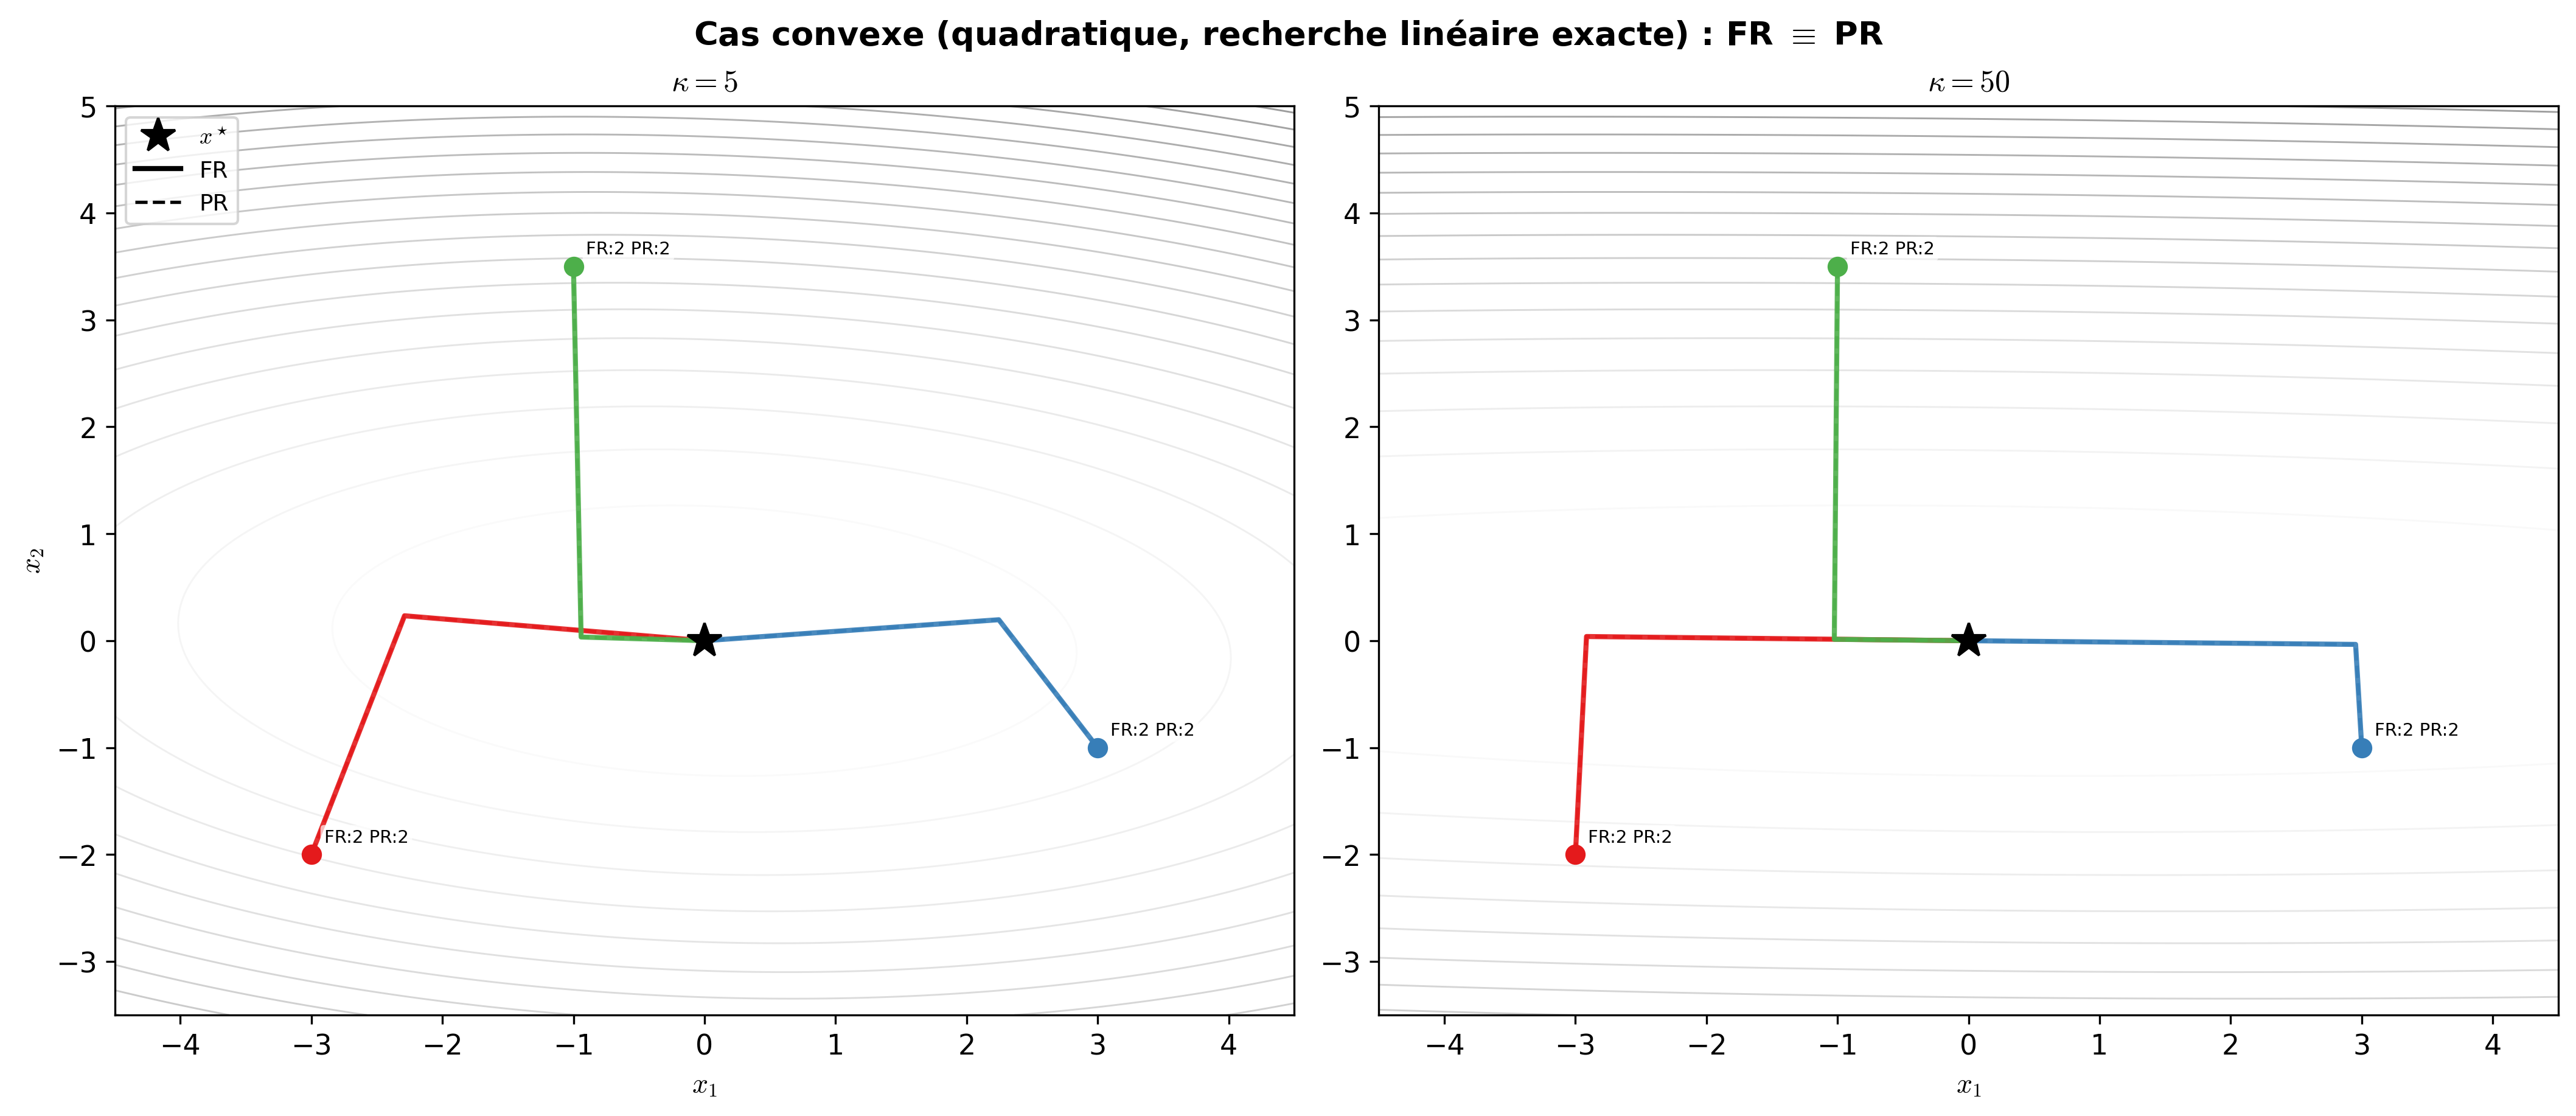
\includegraphics[width=\linewidth]{figures/benchmark2/graphique_1.png}
  \caption{Cas convexe ($f_Q$ en dimension~2 avec recherche linéaire exacte)~: trajectoires FR (trait plein) et PR (pointillés) depuis trois points initiaux (un par couleur). Gauche~: $\kappa = 5$~; droite~: $\kappa = 50$. Les annotations indiquent le nombre d'itérations~; les deux méthodes coïncident dans tous les cas.}
  \label{fig:b2_quad}
\end{figure}

\paragraph{Fonctions multimodales~: bassins d'attraction.}
PR converge systématiquement plus souvent que FR, mais pas vers de meilleurs minima. La figure~\ref{fig:b2_multi} cartographie les bassins d'attraction de $f_M$ sur la grille $50 \times 50$.

\begin{figure}[ht]
  \centering
  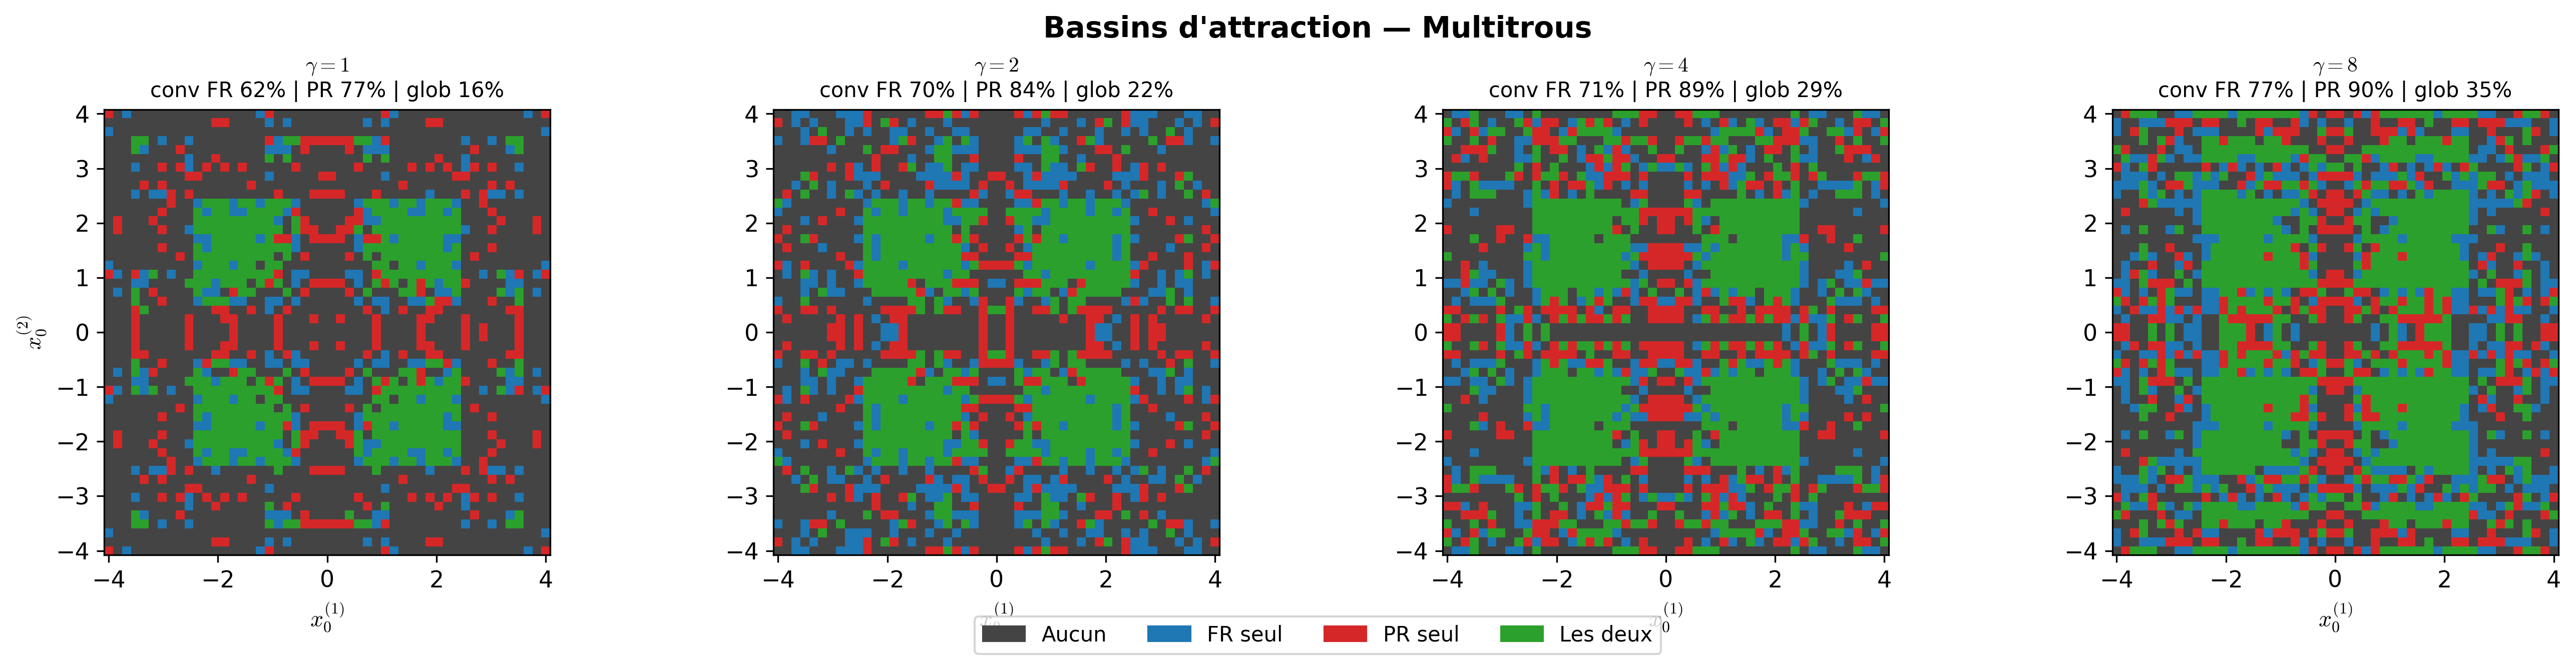
\includegraphics[width=\linewidth]{figures/benchmark2/graphique_2.png}
  \caption{Bassins d'attraction sur la fonction multitrous $f_M$ (grille $50 \times 50$ sur $[-4,4]^2$) pour $\gamma \in \{1, 2, 4, 8\}$. Vert~: les deux méthodes convergent~; bleu~: FR seul~; rouge~: PR seul~; gris~: aucune des deux. Les sous-titres indiquent les taux de convergence de chaque méthode et le taux d'atteinte du minimum global.}
  \label{fig:b2_multi}
\end{figure}

PR affiche un avantage systématique en taux de convergence~: l'écart se maintient entre 13 et 18 points selon $\gamma$ ($62.2\,\%$ contre $77.3\,\%$ à $\gamma = 1$, $77.2\,\%$ contre $90.1\,\%$ à $\gamma = 8$) et ne se résorbe pas lorsque $\gamma$ augmente. L'avantage ne porte toutefois pas sur le minimum \emph{global}~: les deux méthodes l'atteignent dans des proportions comparables (entre $25.8\,\%$ et $54.5\,\%$ selon $\gamma$), et le surplus de convergence de PR se distribue sur les minima \emph{locaux}. Autrement dit, PR ne trouve pas mieux, mais il trouve plus souvent.

L'analyse des modes d'échec éclaire le mécanisme sous-jacent. FR plafonne à la limite de $10^4$ itérations, signe d'une stagnation sans divergence, dans $8.6\,\%$ à $13.6\,\%$ des 2500 exécutions selon $\gamma$, tandis que PR ne stagne quasiment jamais (entre $0.7\,\%$ et $2.6\,\%$). Lorsque PR échoue, il diverge franchement~; lorsque FR échoue, il oscille entre stagnation et divergence à parts comparables. Ce contraste peut s'interpréter à partir de la structure algébrique des deux formules~: $\beta_k^{\text{FR}}$, toujours positif, peut accumuler du moment dans une direction devenue inadaptée après un changement de courbure, maintenant l'itéré dans un voisinage sans progression~; $\beta_k^{\text{PR}}$, dont le numérateur $\langle \nabla f_k,\, \nabla f_k - \nabla f_{k-1} \rangle$ s'annule lorsque les gradients successifs se rapprochent (cas typique de stagnation), tend alors vers $0$ et rabat la direction vers $-\nabla f_k$~: ce comportement peut limiter la stagnation, au prix d'une trajectoire parfois plus erratique.

On observe également une différence dans la diversité de l'exploration. À $\gamma = 1$, les 1933 exécutions convergées de PR atteignent 169 minima locaux distincts, contre 71 pour les 1555 exécutions convergées de FR~; à $\gamma = 8$, le rapport est de 106 contre 50. PR disperse ses trajectoires dans un éventail de bassins sensiblement plus large, là où FR concentre ses convergences sur un sous-ensemble restreint du paysage.

\paragraph{Fonction non bornée~: cas limite de $f_C$.}
La figure~\ref{fig:b2_cubic} reporte les bassins d'attraction sur $f_C$ pour $\gamma \in \{1, 5, 10\}$.

\begin{figure}[ht]
  \centering
  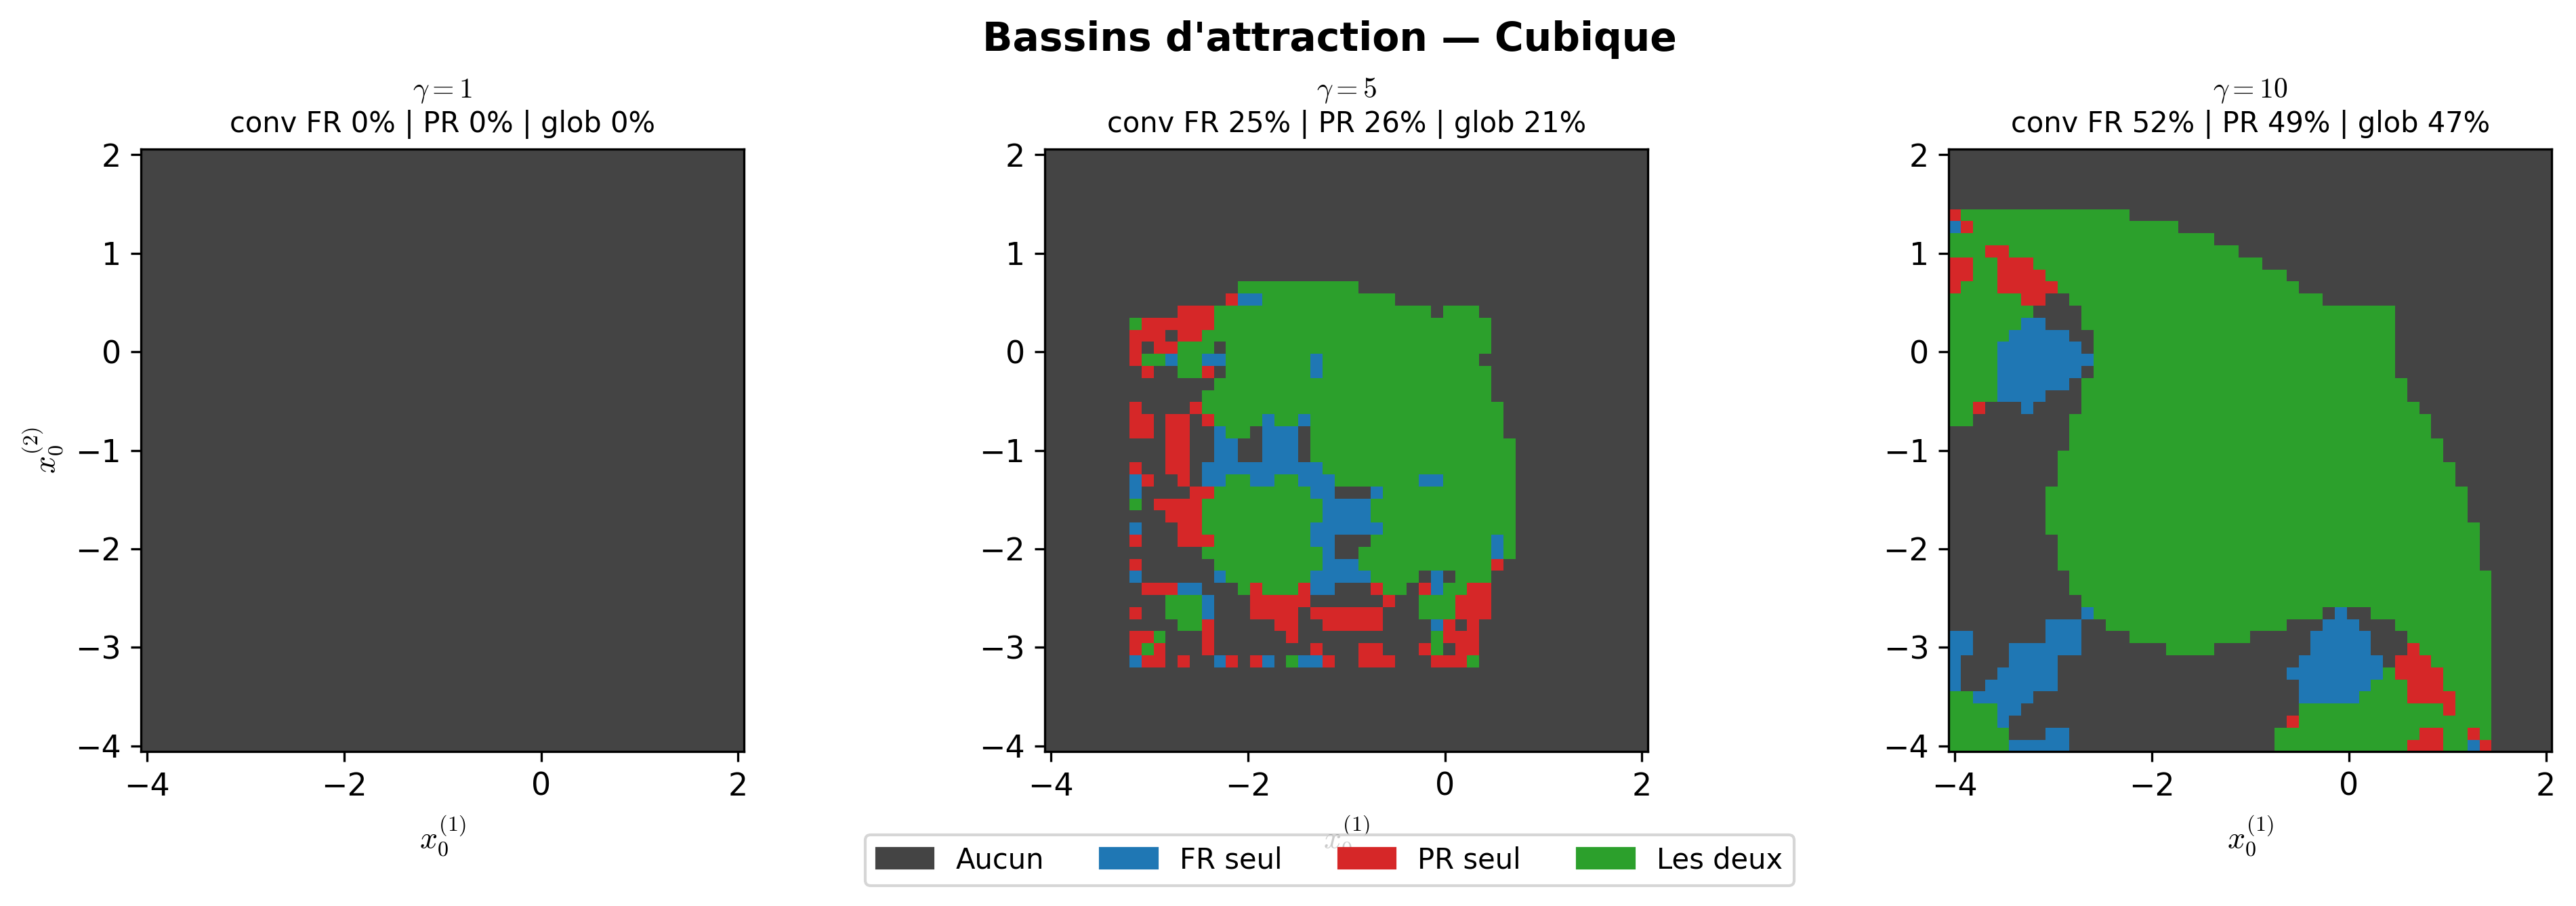
\includegraphics[width=\linewidth]{figures/benchmark2/graphique_3.png}
  \caption{Bassins d'attraction sur la fonction cubique $f_C$ pour $\gamma \in \{1, 5, 10\}$. Même code couleur que la figure~\ref{fig:b2_multi}. À $\gamma = 1$, l'absence de point critique rend le panneau uniformément gris. À $\gamma \in \{5, 10\}$, le bassin de convergence (vert) s'élargit avec $\gamma$.}
  \label{fig:b2_cubic}
\end{figure}

Le cas $\gamma = 1$ constitue un test de robustesse à la divergence~: le discriminant de la dérivée de chaque composante est négatif ($4\gamma^2 - 12 = -8$), la fonction n'admet aucun point critique et décroît sans borne. Les deux méthodes divergent sur la totalité des 2500 points initiaux, confirmant le bon fonctionnement de ce test de divergence. À $\gamma = 5$, un minimum local apparaît en $(-0.103,\, -0.103)$ et les taux de convergence restent faibles mais comparables~: $24.8\,\%$ pour FR, $26.2\,\%$ pour PR. À $\gamma = 10$, le puits se creuse et le bassin s'élargit~: $51.9\,\%$ pour FR, $48.5\,\%$ pour PR~; les positions finales des exécutions convergées coïncident avec le minimum local analytique. Contrairement à $f_M$, la difficulté ne provient pas ici de la multiplicité des minima mais de l'absence de borne inférieure~: toute trajectoire quittant le bassin du minimum local est aspirée vers $-\infty$ par le terme cubique dominant. Dans ce régime, le choix FR contre PR n'apporte pas d'avantage mesurable~; c'est la géométrie du bassin, et non la formule de $\beta_k$, qui détermine l'issue.

\paragraph{Vitesse de convergence conditionnelle.}
Sur $f_M$, PR est systématiquement plus rapide en médiane~: 27 itérations contre 38 pour FR à $\gamma = 1$, 24 contre 54 à $\gamma = 8$, soit un ratio FR/PR qui croît de $1.4$ à $2.25$ (figure~\ref{fig:b2_box}).

\begin{figure}[ht]
  \centering
  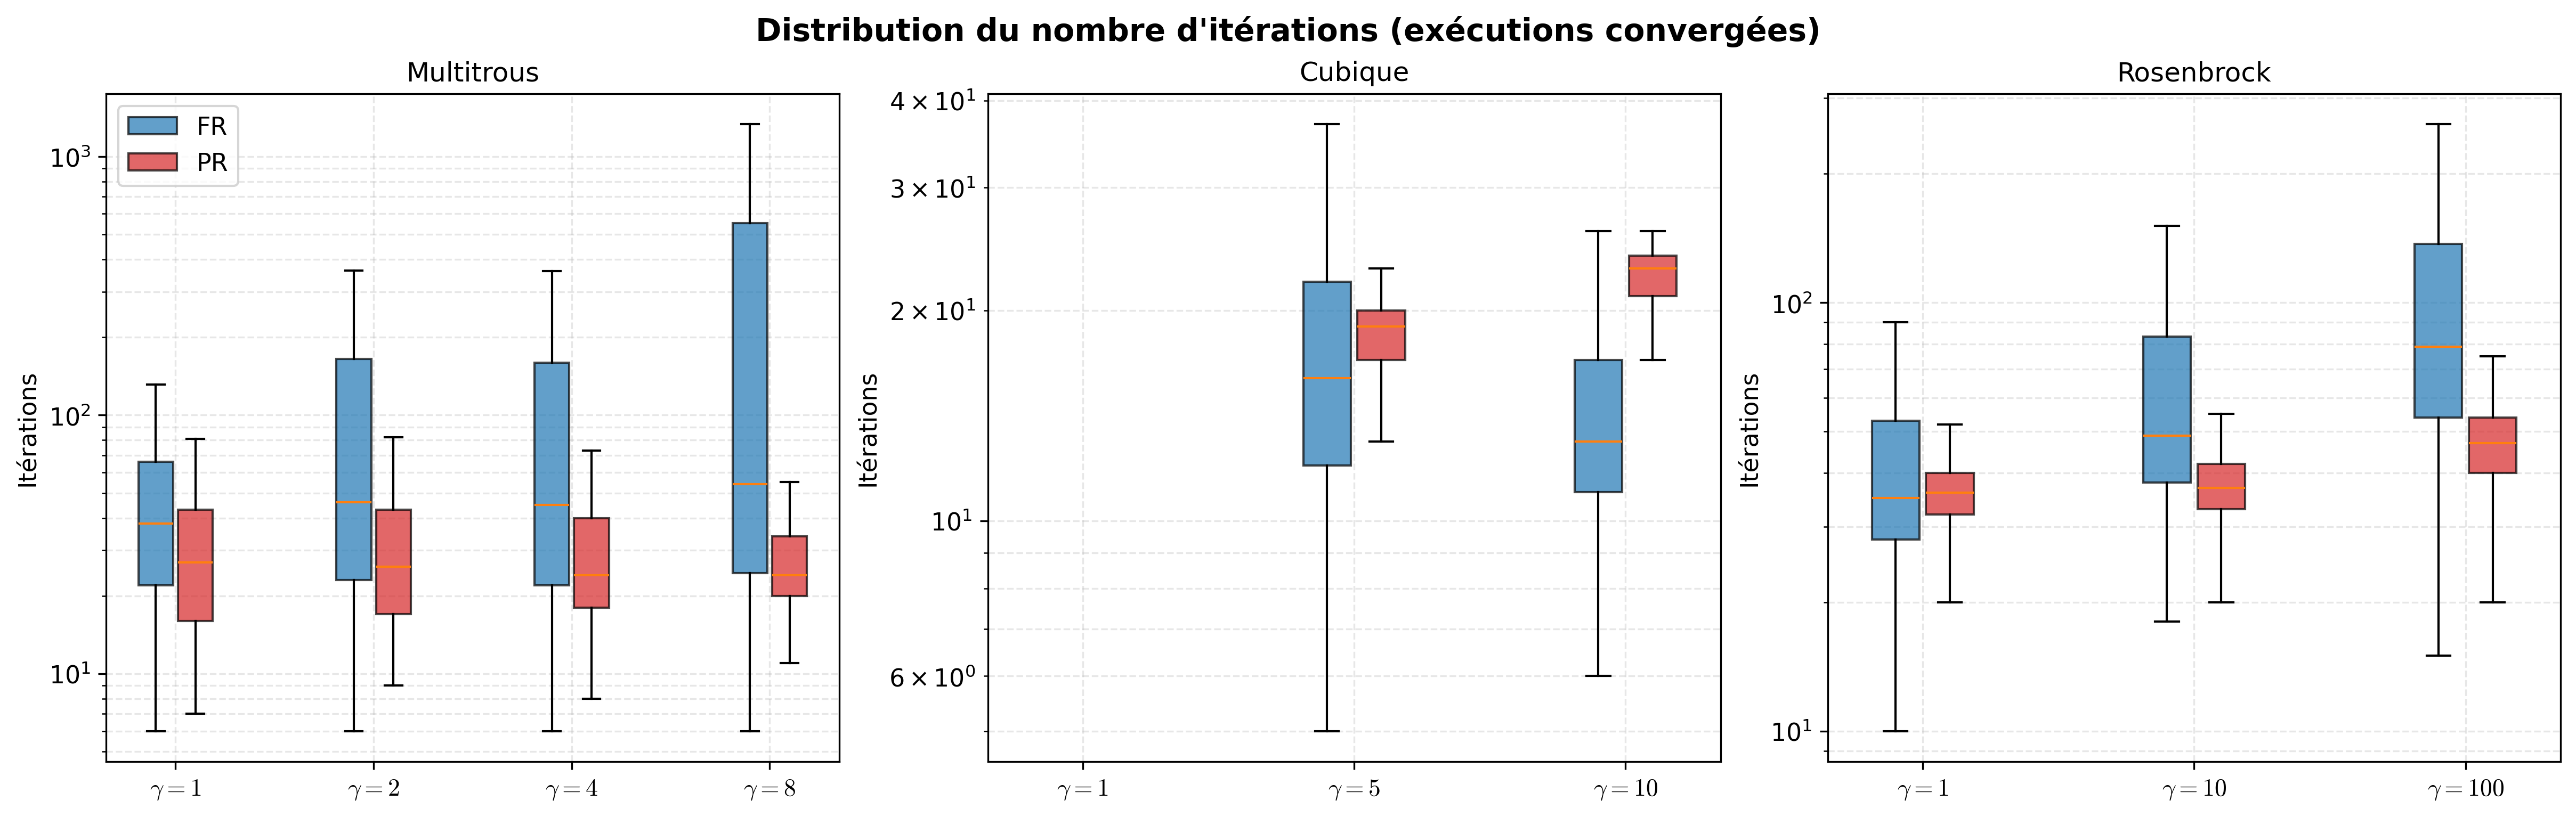
\includegraphics[width=\linewidth]{figures/benchmark2/graphique_4.png}
  \caption{Distribution du nombre d'itérations parmi les exécutions convergées. De gauche à droite~: multitrous ($\gamma \in \{1, 2, 4, 8\}$), cubique ($\gamma \in \{1, 5, 10\}$), Rosenbrock ($\gamma \in \{1, 10, 100\}$). Bleu~: FR~; rouge~: PR.}
  \label{fig:b2_box}
\end{figure}

La différence la plus frappante ne réside toutefois pas dans la médiane mais dans la dispersion. À $\gamma = 8$, l'intervalle interquartile de FR s'étend de 24 à 552 itérations, soit un facteur 23~; celui de PR, de 20 à 34, soit un facteur~$1.7$. La moyenne de FR atteint 836 itérations, soit $15.5$ fois sa médiane, signature d'une queue de distribution extrêmement lourde. Concrètement, une fraction non négligeable des exécutions FR convergées nécessitent plusieurs centaines, voire plusieurs milliers d'itérations pour aboutir, là où PR termine en quelques dizaines d'itérations dans la quasi-totalité des cas. Cette asymétrie s'interprète comme un artefact de la stagnation partielle de FR~: certaines exécutions finissent par converger après une longue phase d'oscillation, mais au prix d'un surcoût considérable en itérations.

Sur la fonction de Rosenbrock, les deux méthodes convergent dans $100\,\%$ des cas, mais leur vitesse se différencie progressivement avec $\gamma$. À $\gamma = 1$, les médianes sont quasi-identiques (35 contre 36) et PR ne l'emporte que dans $50.7\,\%$ des points initiaux~: les deux méthodes sont effectivement équivalentes, en cohérence avec la faible non-linéarité du problème. À $\gamma = 100$, la situation bascule~: FR atteint une médiane de 79 itérations (IQR $[54,\, 137]$) contre 47 pour PR (IQR $[40,\, 54]$), et PR converge plus vite dans $84.3\,\%$ des points initiaux. La direction héritée de FR, qui accumule du moment le long de l'axe principal de la vallée, se retrouve périodiquement en porte-à-faux par rapport au gradient local lorsque la courbure transverse est forte~; la prise en compte de la variation du gradient par PR peut aider à corriger cette dérive.

La figure~\ref{fig:b2_traj} illustre cette différence de comportement sur trois points initiaux choisis pour maximiser l'écart d'itérations entre les deux méthodes.

\begin{figure}[ht]
  \centering
  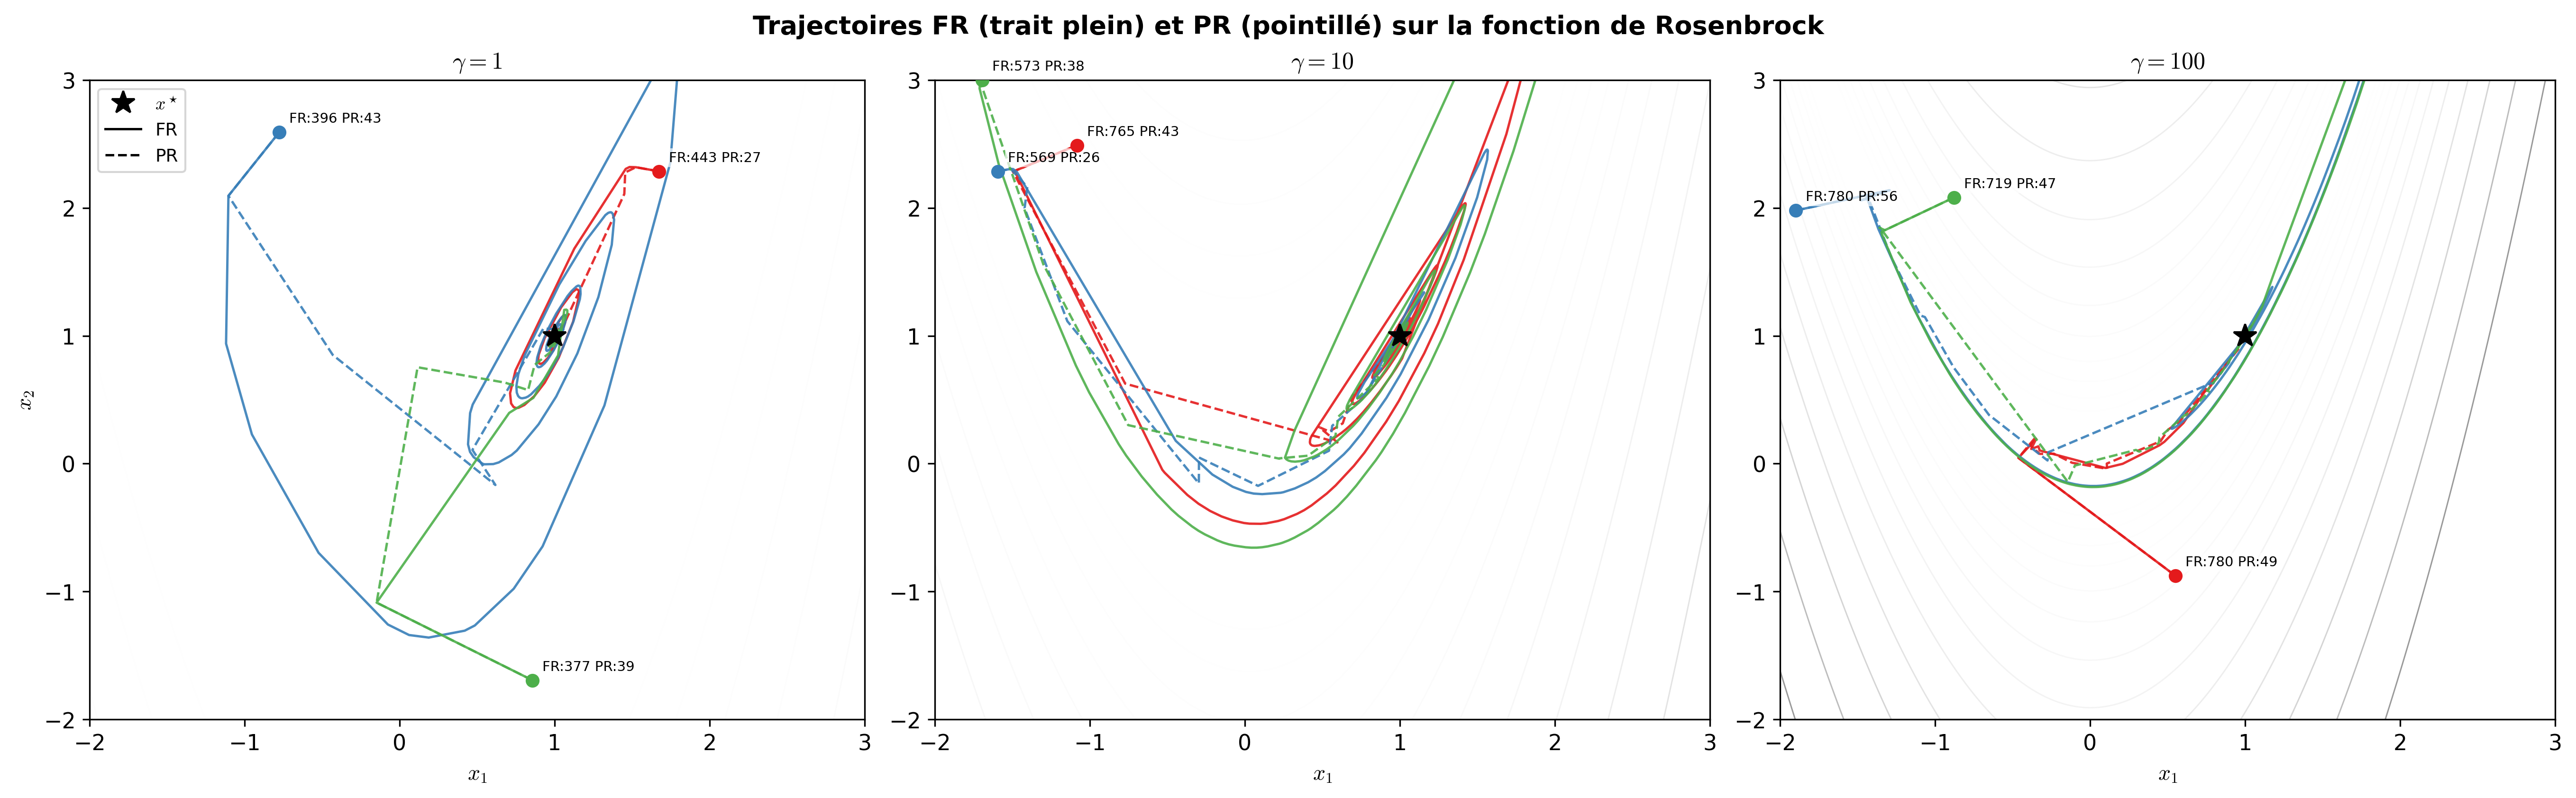
\includegraphics[width=\linewidth]{figures/benchmark2/graphique_5.png}
  \caption{Trajectoires FR (trait plein) et PR (pointillés) sur la fonction de Rosenbrock pour $\gamma \in \{1, 10, 100\}$ (un panneau par valeur de $\gamma$), depuis trois points initiaux (un par couleur) choisis pour maximiser l'écart d'itérations entre les deux méthodes. Les annotations indiquent le nombre d'itérations de chaque méthode~; les lignes de niveau de $f_R$ figurent en arrière-plan.}
  \label{fig:b2_traj}
\end{figure}

\paragraph{Synthèse.}
Sur la fonction quadratique avec recherche linéaire exacte, FR et PR coïncident rigoureusement. Sur les fonctions non-convexes avec critère d'Armijo, PR se distingue sur deux axes. En \emph{robustesse} d'abord~: son taux de convergence dépasse celui de FR de 13 à 18 points sur $f_M$, et ses échecs prennent la forme d'une divergence franche plutôt que d'une stagnation prolongée. En \emph{vitesse} ensuite~: le ratio médian d'itérations FR/PR atteint $2.25$ sur $f_M$ à $\gamma = 8$ et $1.68$ sur $f_R$ à $\gamma = 100$, avec une dispersion de FR considérablement plus large (rapport moyen/médiane jusqu'à $15.5$). Le mécanisme unificateur est le signe de $\beta_k$~: toujours positif pour FR, ce qui prolonge le moment dans des directions devenues inadaptées~; potentiellement négatif pour PR, ce qui permet d'inverser la contribution de la direction précédente lorsque celle-ci devient inadaptée, sans nécessiter de critère de redémarrage explicite.

\newpage

\subsection{Benchmark 3~: Gradient conjugué, Newton et BFGS}\label{sec:b3}

\subsubsection{Protocole expérimental}

Ce benchmark confronte trois méthodes d'ordres de convergence différents~: gradient conjugué~-~Polak-Ribière (CG-PR), Newton et quasi-Newton (BFGS), dans deux régimes séparés.

\paragraph{Régime quadratique.} Sur la fonction $f_Q$, les trois méthodes sont comparées. Newton utilise la direction $d_k = -A^{-1}\nabla f(x_k)$ avec un pas $\eta = 1$ (sans recherche linéaire, le modèle quadratique étant exact)~; la matrice $A^{-1}$ est précalculée une seule fois. CG-PR et BFGS utilisent la recherche d'Armijo avec $(\alpha, \beta) = (0.25, 0.5)$, le même critère d'arrêt $\|\nabla f(x_k)\| < 10^{-6}$, et la même limite de $10^4$ itérations. On parcourt $n \in \{2, 5, 10, 50, 100\}$ et $\kappa \in \{5, 10, 50, 100, 500\}$. Pour chaque combinaison $(n, \kappa)$, 20 matrices sont générées par \texttt{create\_system(n, cond=$\kappa$, seed=s)} pour $s \in \{0, \ldots, 19\}$, avec $x_0 = 0$. La solution exacte $x^\star = A^{-1}b$ permet de mesurer l'erreur $\|x_k - x^\star\|_2$ à chaque itération.

\paragraph{Régime général.} La méthode de Newton est inapplicable (la hessienne n'est pas connue analytiquement), et l'on compare uniquement CG-PR et BFGS. Les fonctions testées sont la fonction de Rosenbrock $f_R$ avec $\gamma \in \{1, 10, 100\}$ et la fonction multitrous $f_M$ avec $\gamma \in \{1, 2, 4, 8\}$. Pour chaque couple (fonction, $\gamma$), 20 points initiaux sont tirés uniformément dans le domaine pertinent (graine fixe). Les métriques collectées sont le nombre d'itérations, le nombre total d'évaluations de $f$ et l'erreur finale $\|x_{\text{final}} - x^\star\|$ lorsque $x^\star$ est connu. Les statistiques sont agrégées par médiane et intervalle interquartile sur les 20 instances.

\subsubsection{Résultats et Analyse}

L'analyse s'organise en six temps. On vérifie d'abord la convergence en une itération de Newton sur la fonction quadratique. On caractérise ensuite la sensibilité comparée des trois méthodes à la dimension et au conditionnement. L'ordre de convergence empirique est ensuite estimé quantitativement. On confronte alors le coût en itérations au coût en évaluations de $f$. On étudie le régime général sur la fonction de Rosenbrock et la fonction multitrous, avant de dégager une synthèse.

\paragraph{Convergence de Newton en une itération.}
Sur les 25 combinaisons $(n, \kappa)$ et les 20 matrices par combinaison, soit 500 exécutions au total, Newton converge systématiquement en une seule itération, avec un taux de convergence de $100\,\%$. L'erreur finale est de l'ordre de la précision machine ($\sim 10^{-15}$). Sur $f_Q$, la direction de Newton est $d_0 = -A^{-1}(Ax_0 - b) = x^\star - x_0$ et le pas $\eta = 1$ amène directement à $x^\star$. Le fait que ce résultat tienne indifféremment à $n = 2$ et $n = 100$, à $\kappa = 5$ et $\kappa = 500$, confirme l'insensibilité totale de Newton à la dimension et au conditionnement sur cette classe de fonctions. Le prix est l'accès à $A^{-1}$, qui coûte $O(n^3)$ en calcul.

\paragraph{Sensibilité à la dimension et au conditionnement.}
CG-PR dépasse généralement la borne théorique de $n$ itérations valable avec recherche linéaire exacte (figure~\ref{fig:b3_dim}).

\begin{figure}[H]
  \centering
  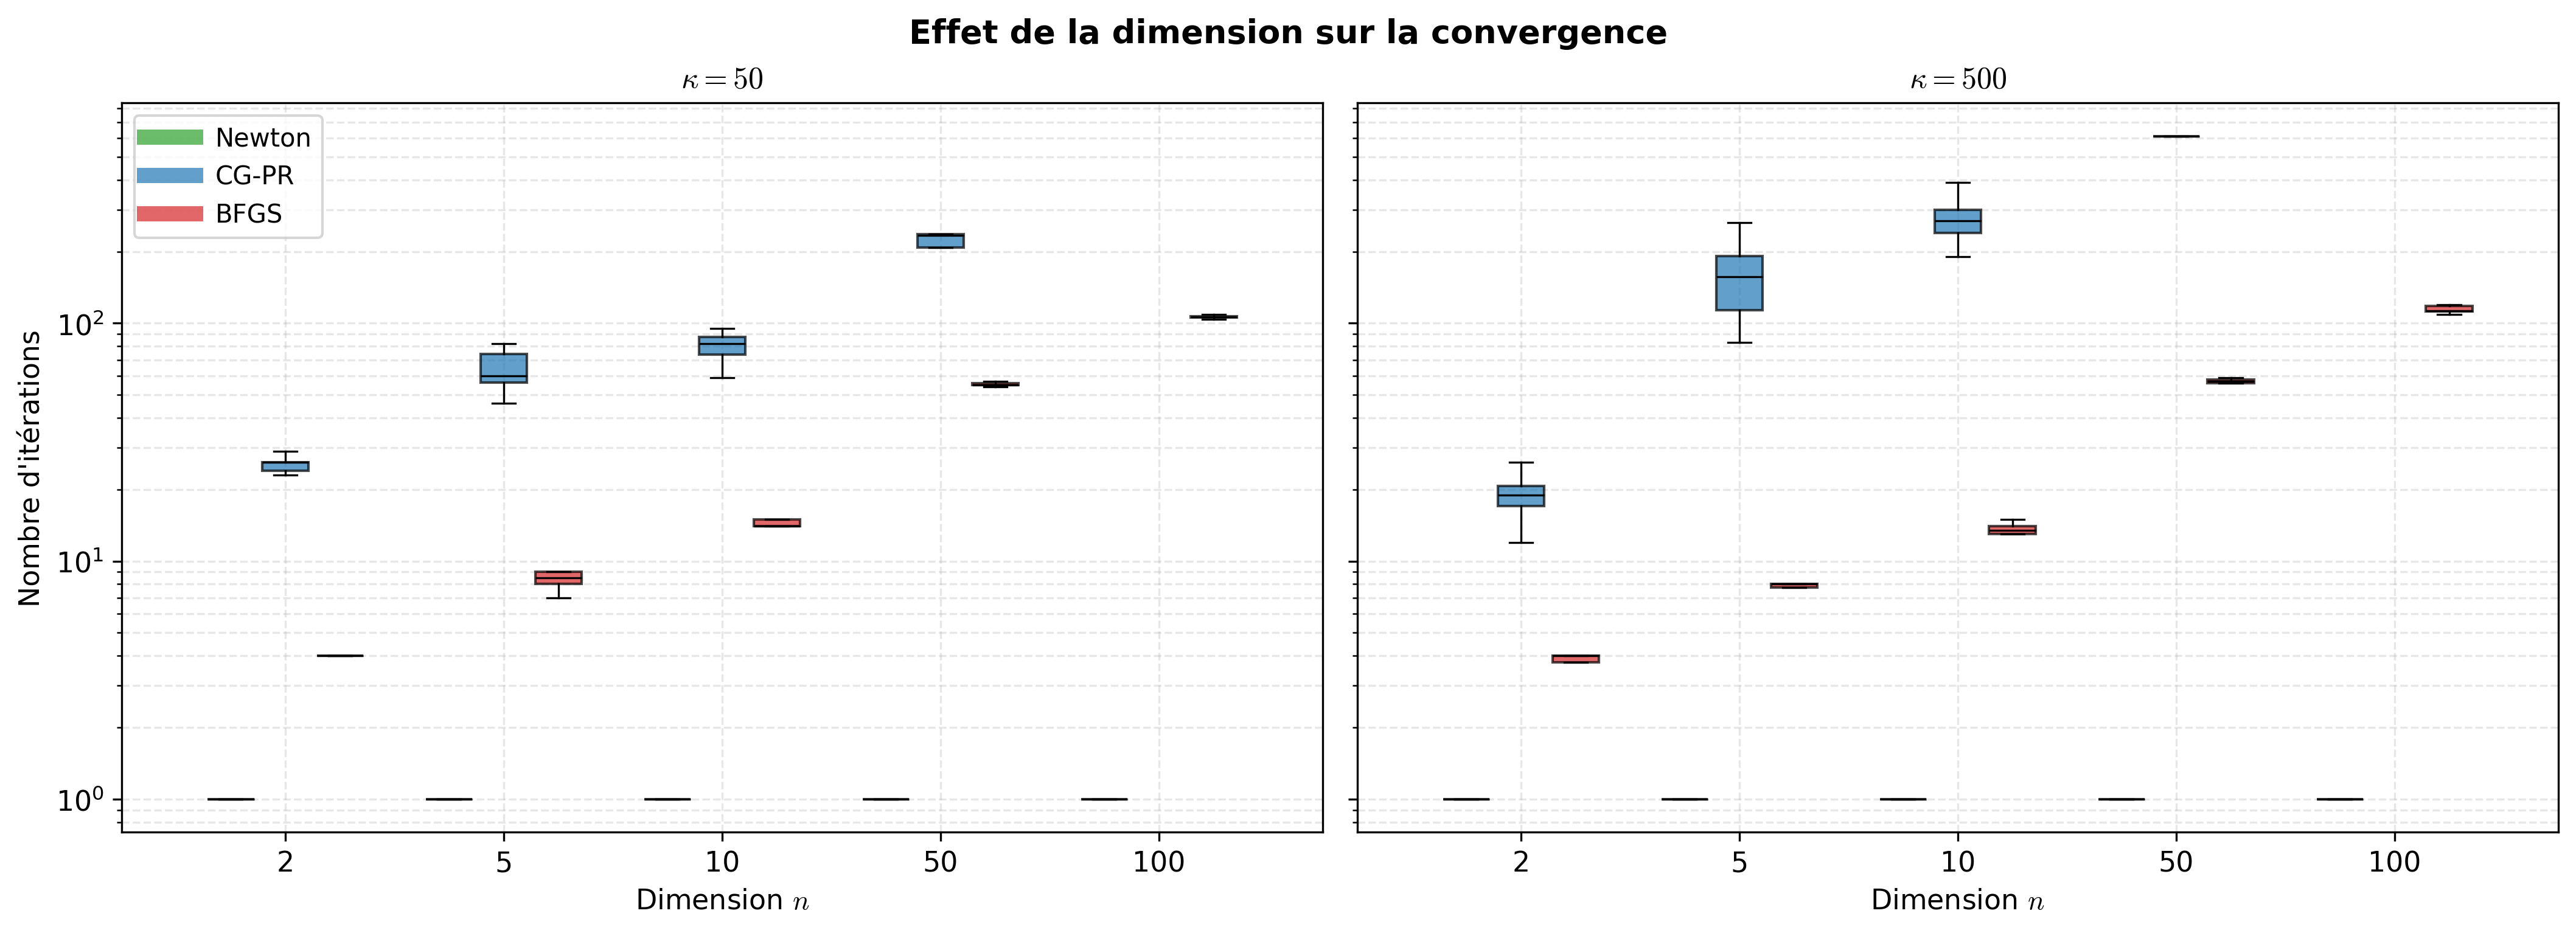
\includegraphics[width=\linewidth]{figures/benchmark3/fig1_scaling_dim.png}
  \caption{Effet de la dimension sur la convergence~: nombre d'itérations en fonction de $n$ (boxplots sur 20 graines). Gauche~: $\kappa = 50$~; droite~: $\kappa = 500$. Newton (vert) converge invariablement en 1 itération~; CG-PR (bleu) croît avec $n$ et $\kappa$~; BFGS (rouge) croît avec $n$ et sa sensibilité à $\kappa$ reste faible jusqu'à $n = 50$ avant d'apparaître à $n = 100$ (échec à $\kappa = 500$).}
  \label{fig:b3_dim}
\end{figure}

À $n = 10$ et $\kappa = 50$, la médiane est de 82 itérations, soit $8.2$ fois la dimension~; à $\kappa = 500$, elle monte à 270 itérations (27 fois $n$), avec un taux de convergence qui chute à $70\,\%$. À grande dimension, la dégradation s'amplifie~: à $n = 100$, CG-PR ne converge plus qu'à $70\,\%$ pour $\kappa = 5$ et à $40\,\%$ pour $\kappa = 10$, et échoue totalement dès $\kappa \geq 50$.

\begin{figure}[H]
  \centering
  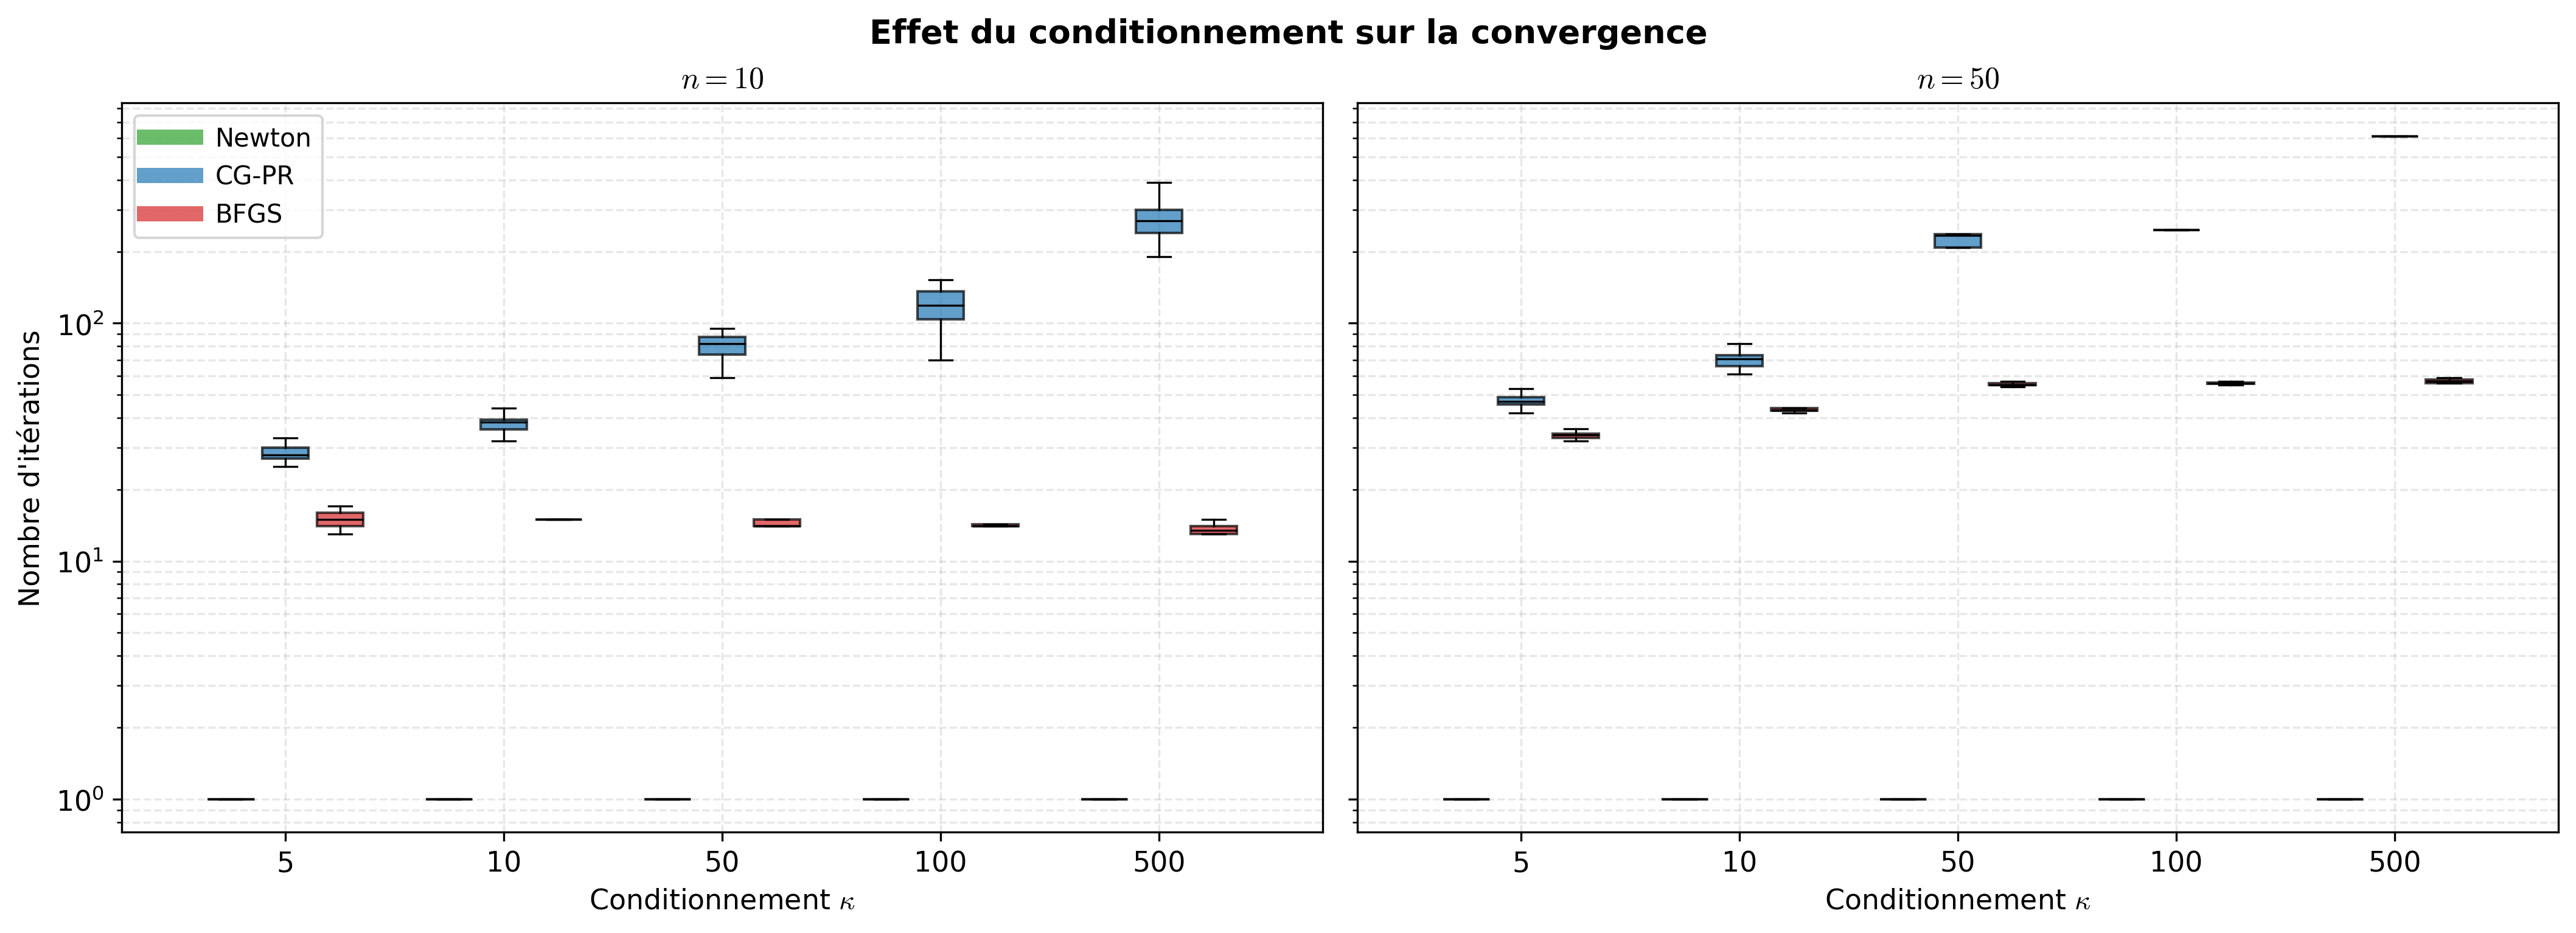
\includegraphics[width=\linewidth]{figures/benchmark3/fig2_scaling_kappa.png}
  \caption{Effet du conditionnement sur la convergence~: nombre d'itérations en fonction de $\kappa$ (boxplots sur 20 graines). Gauche~: $n = 10$~; droite~: $n = 50$. Même code couleur que la figure~\ref{fig:b3_dim}. L'insensibilité de BFGS au conditionnement (médiane de 13 à 15 itérations sur toute la plage de $\kappa$ à $n = 10$) contraste avec la dégradation quasi-linéaire de CG-PR.}
  \label{fig:b3_kappa}
\end{figure}

BFGS est quasi-insensible au conditionnement \emph{à petite dimension}~: à $n = 10$, sa médiane varie de 13 à 15 itérations sur l'ensemble de la plage $\kappa \in [5, 500]$ (figure~\ref{fig:b3_kappa}). Cette insensibilité s'explique par la mise à jour de rang~2 de $H_k$~: dès que la matrice approchée capture les directions principales de courbure, la convergence asymptotique super-linéaire ne dépend plus du rapport des valeurs propres extrêmes. CG-PR est en revanche sensible à $\kappa$ dès $n = 10$~: sa médiane passe de 28 à 270 itérations entre $\kappa = 5$ et $\kappa = 500$.

Cette insensibilité s'estompe toutefois à grande dimension. BFGS procède en deux phases~: une phase transitoire pendant laquelle $H_k$, initialisée à $I$, reconstruit l'information de courbure (donc $\kappa$-dépendante), puis une phase super-linéaire insensible à $\kappa$. Empiriquement, cette phase transitoire croît linéairement avec $n$ (cohérent avec le fait que $H_k$ doit accumuler $\sim n$ mises à jour de rang~2 avant d'approcher $A^{-1}$). À $n = 10$, elle représente $\sim 10$ itérations sur 13--15~: la phase super-linéaire domine et masque l'effet de $\kappa$. À $n = 50$ et $n = 100$, la phase transitoire devient le coût dominant et la sensibilité à $\kappa$ réapparaît~: la médiane passe de 34 à 58 itérations entre $\kappa = 5$ et $\kappa = 500$ à $n = 50$ (+70\,\%), et de 60 à 109 entre $\kappa = 5$ et $\kappa = 100$ à $n = 100$ (BFGS échoue ensuite à $\kappa = 500$).

\paragraph{Ordre de convergence empirique.}

La figure~\ref{fig:b3_conv} reporte les courbes de convergence $\|x_k - x^\star\|_2$ en fonction des itérations pour les trois méthodes à $n = 10$. Newton apparaît comme une ligne verticale (passage de $\|x_0 - x^\star\|$ à $\sim 10^{-15}$ en une seule itération). Les trajectoires de CG-PR présentent une allure géométrique régulière en échelle semi-logarithmique~; celles de BFGS accélèrent visiblement, signe d'un ordre de convergence supérieur à~1.

\begin{figure}[H]
  \centering
  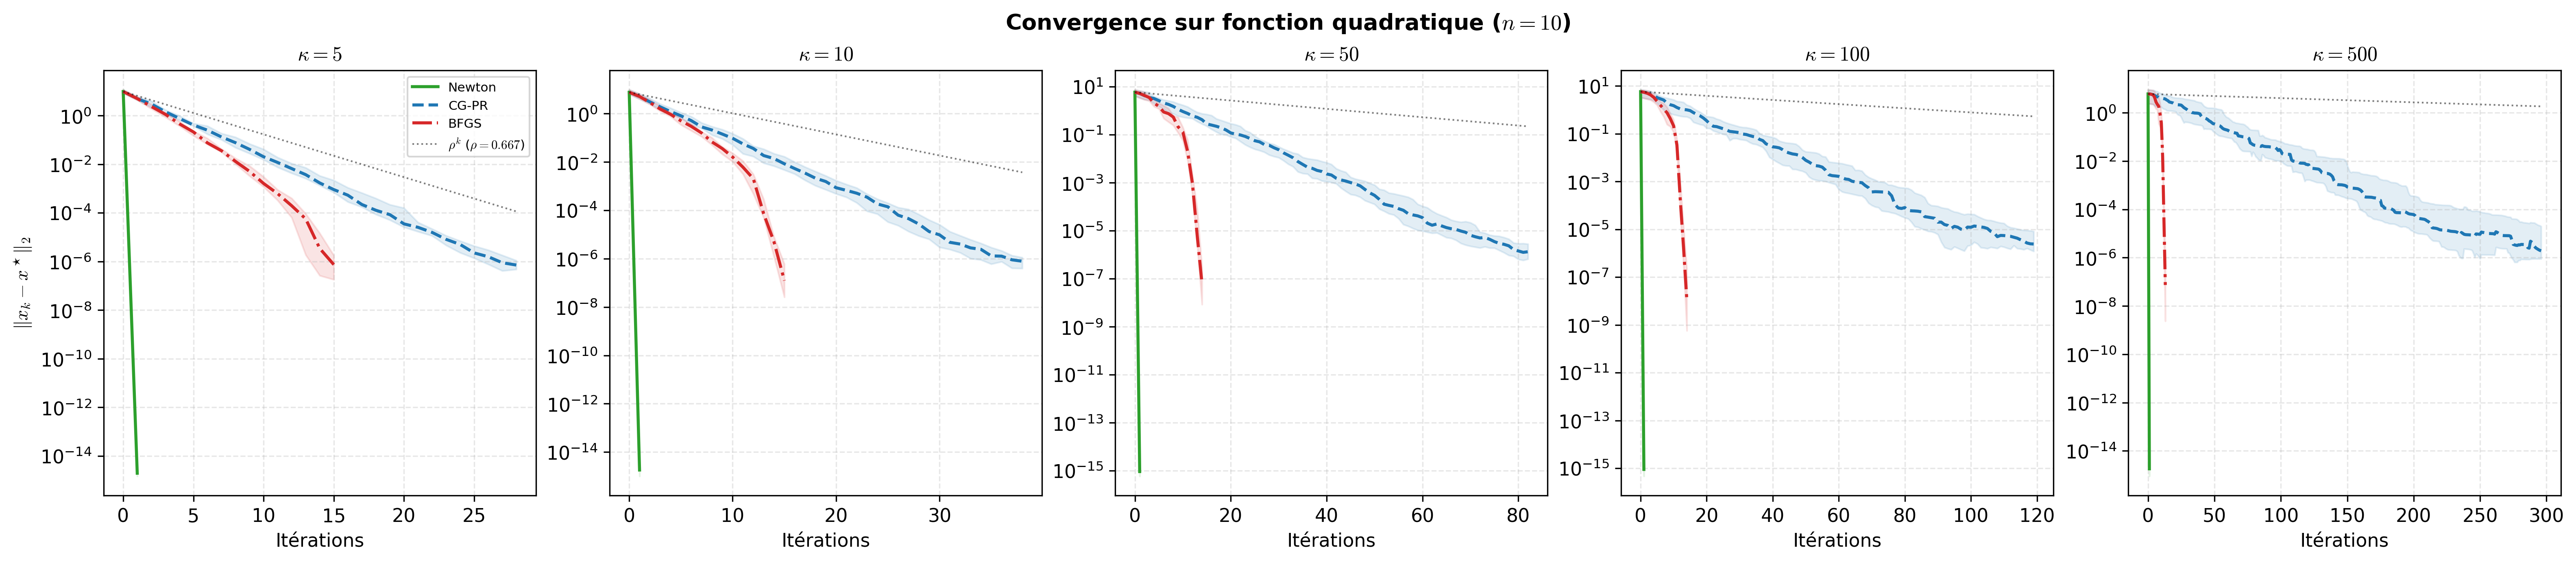
\includegraphics[width=\linewidth]{figures/benchmark3/fig3_convergence_quad.png}
  \caption{Convergence sur la fonction quadratique ($n = 10$)~: $\|x_k - x^\star\|_2$ en fonction de $k$ pour Newton (vert), CG-PR (bleu) et BFGS (rouge), médiane $\pm$ IQR sur 20 graines. De gauche à droite~: $\kappa \in \{5, 10, 50, 100, 500\}$. La borne théorique $\rho^k$ est superposée en pointillés.}
  \label{fig:b3_conv}
\end{figure}

La figure~\ref{fig:b3_order} quantifie cette observation. Pour chaque paire consécutive $(e_k, e_{k+1})$ de l'ensemble des graines, on trace $\log_{10}\|e_{k+1}\|$ en fonction de $\log_{10}\|e_k\|$. Une convergence d'ordre $p$ se traduit par une pente de $p$ dans ce plan.

\begin{figure}[H]
  \centering
  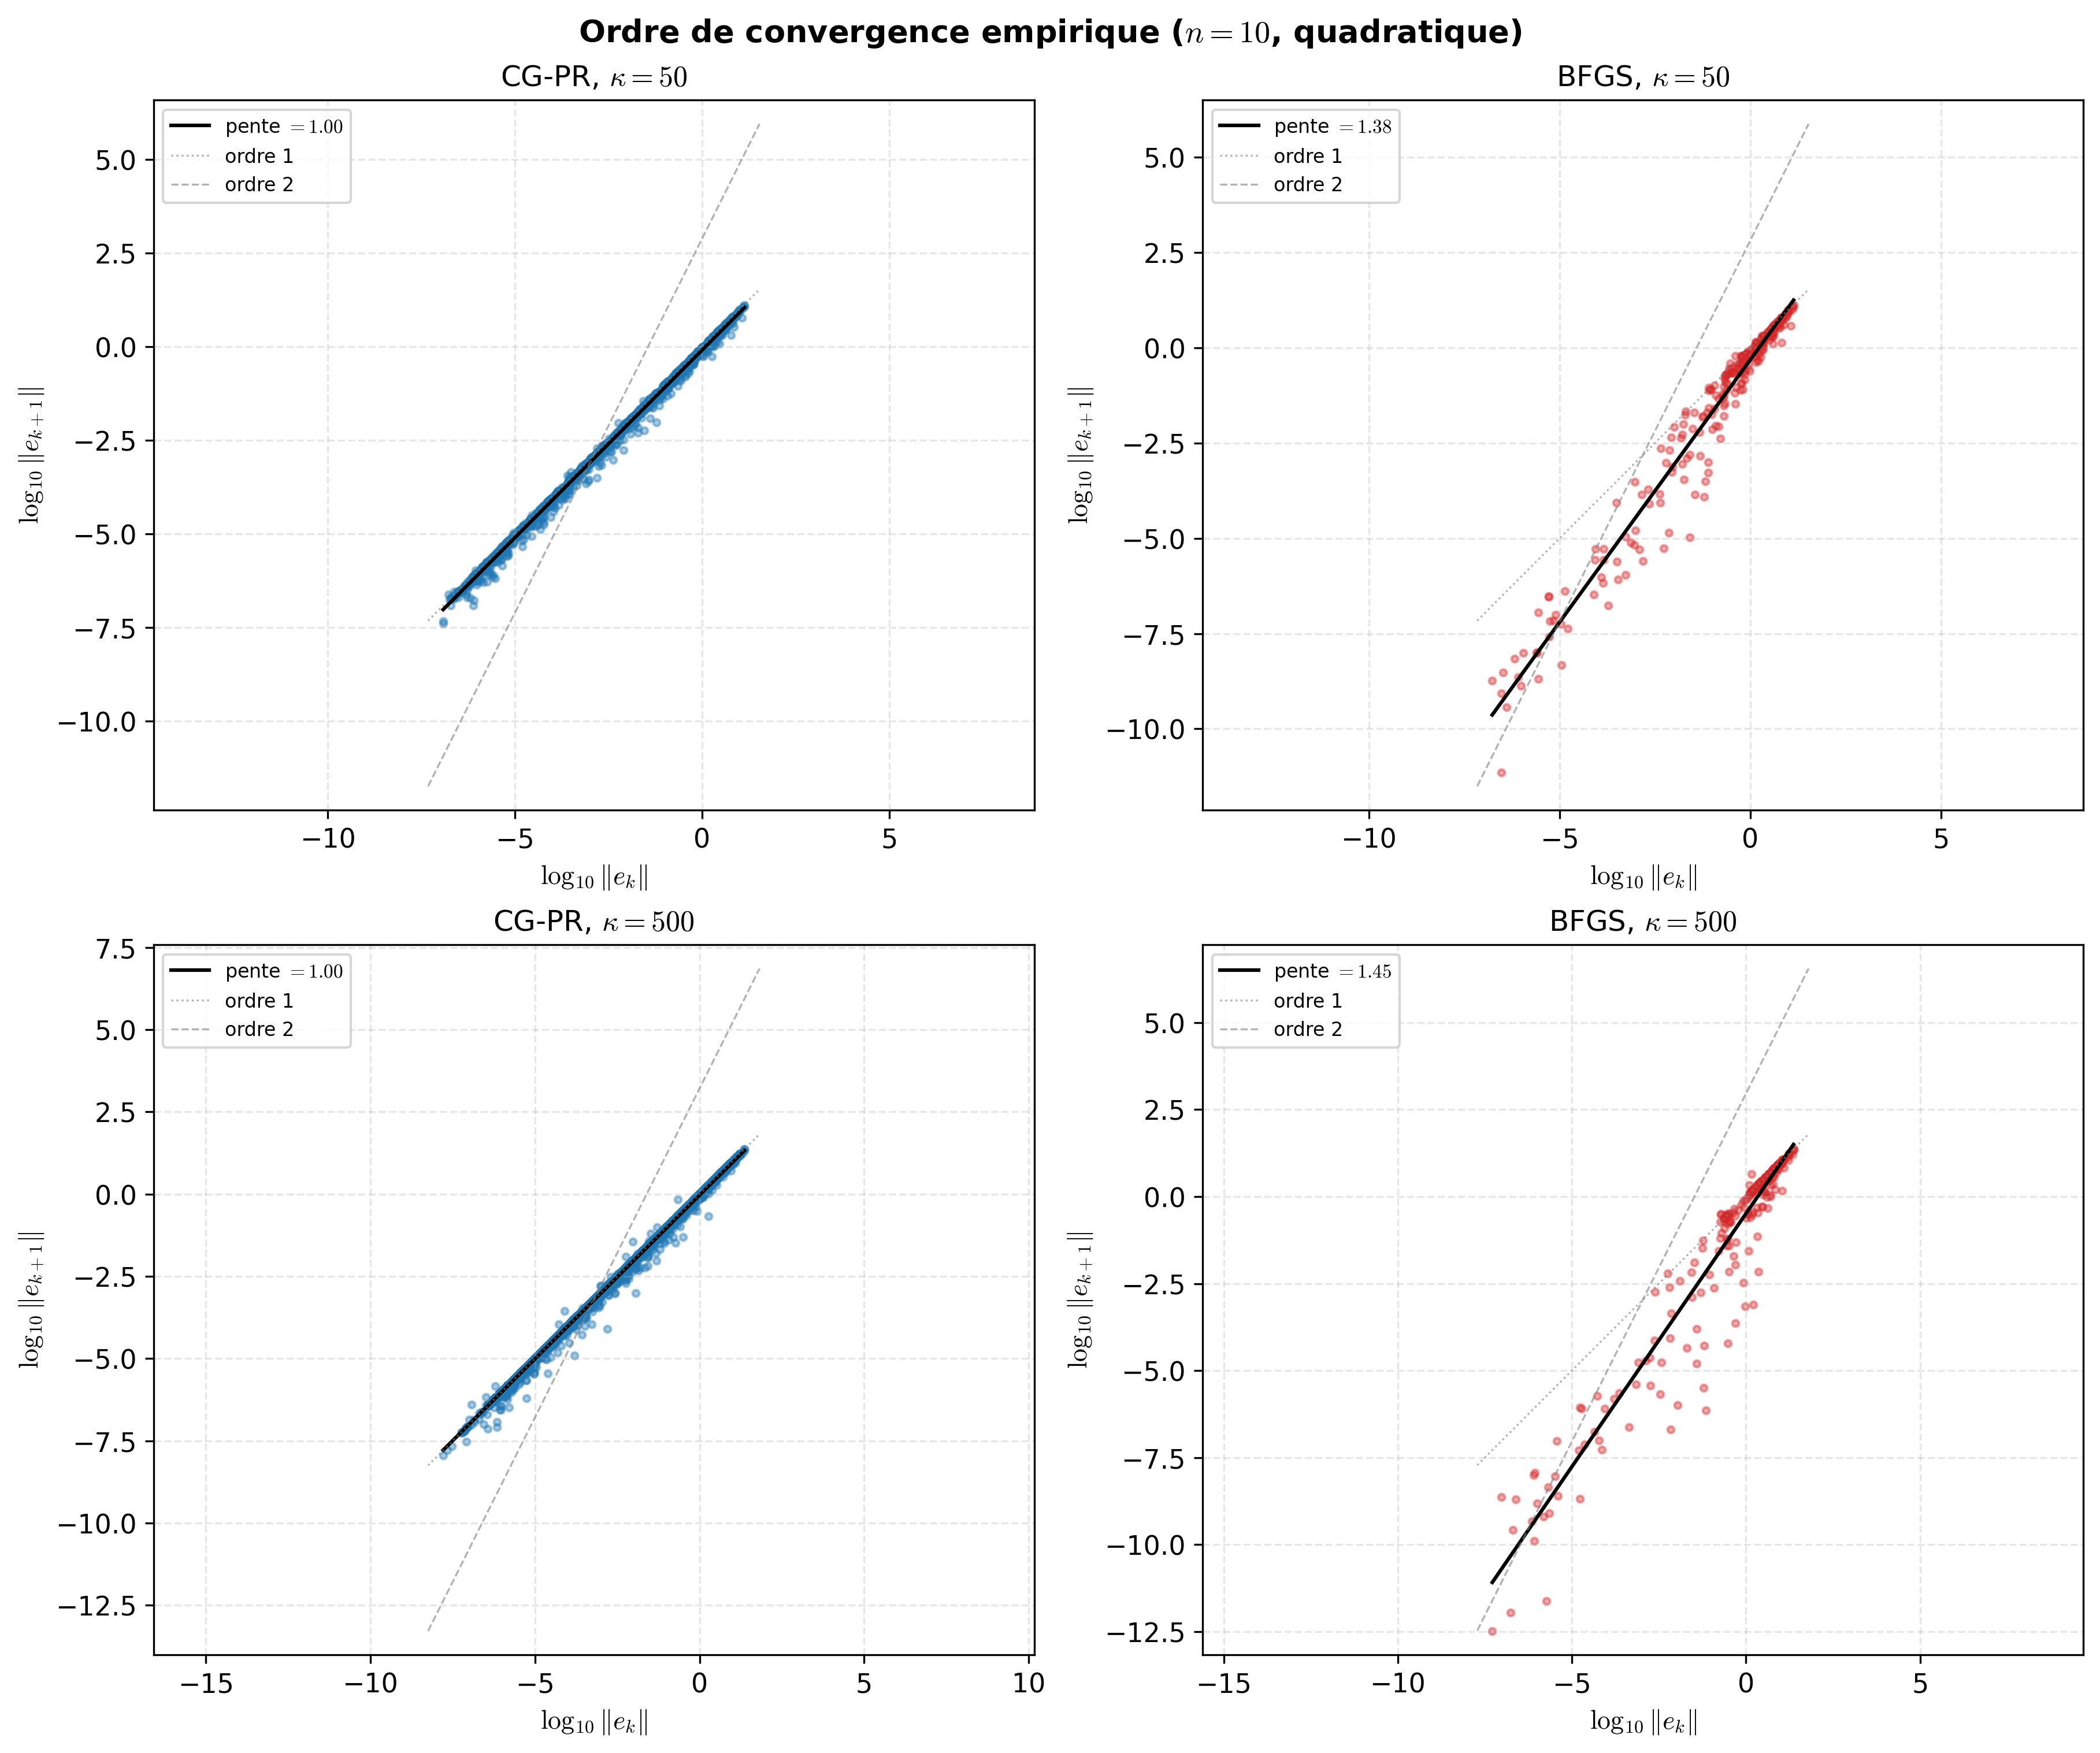
\includegraphics[width=\linewidth]{figures/benchmark3/fig4_convergence_order.png}
  \caption{Ordre de convergence empirique ($n = 10$, fonction quadratique)~: $\log_{10}\|e_{k+1}\|$ en fonction de $\log_{10}\|e_k\|$. Grille $2 \times 2$~: CG-PR à gauche, BFGS à droite~; $\kappa = 50$ en haut, $\kappa = 500$ en bas. Les droites de référence d'ordre~1 et d'ordre~2 sont superposées en gris. CG-PR~: pente $= 1.00$ (linéaire). BFGS~: pente comprise entre $1.14$ et $1.45$.}
  \label{fig:b3_order}
\end{figure}

CG-PR affiche une pente de $1.00$ à tous les conditionnements testés, suggérant une convergence linéaire~: le nuage de points s'aligne exactement sur la droite de référence d'ordre~1. BFGS présente des pentes allant de $1.14$ à $\kappa = 5$ jusqu'à $1.45$ à $\kappa = 500$, suggérant une convergence super-linéaire, en accord avec la théorie. L'augmentation apparente de l'ordre empirique avec $\kappa$ est un artefact de l'estimation~: la pente est ajustée sur l'ensemble de la trajectoire, qui mélange une phase transitoire lente ($\kappa$-dépendante) et une phase asymptotique super-linéaire. À $\kappa$ élevé, le contraste entre les deux phases s'accentue, ce qui gonfle la pente unique ajustée.

\paragraph{Coût réel~: évaluations de $f$.}
La figure~\ref{fig:b3_cost} confronte le nombre d'itérations (coût apparent) au nombre total d'évaluations de $f$ (coût réel) à $n = 10$.

\begin{figure}[H]
  \centering
  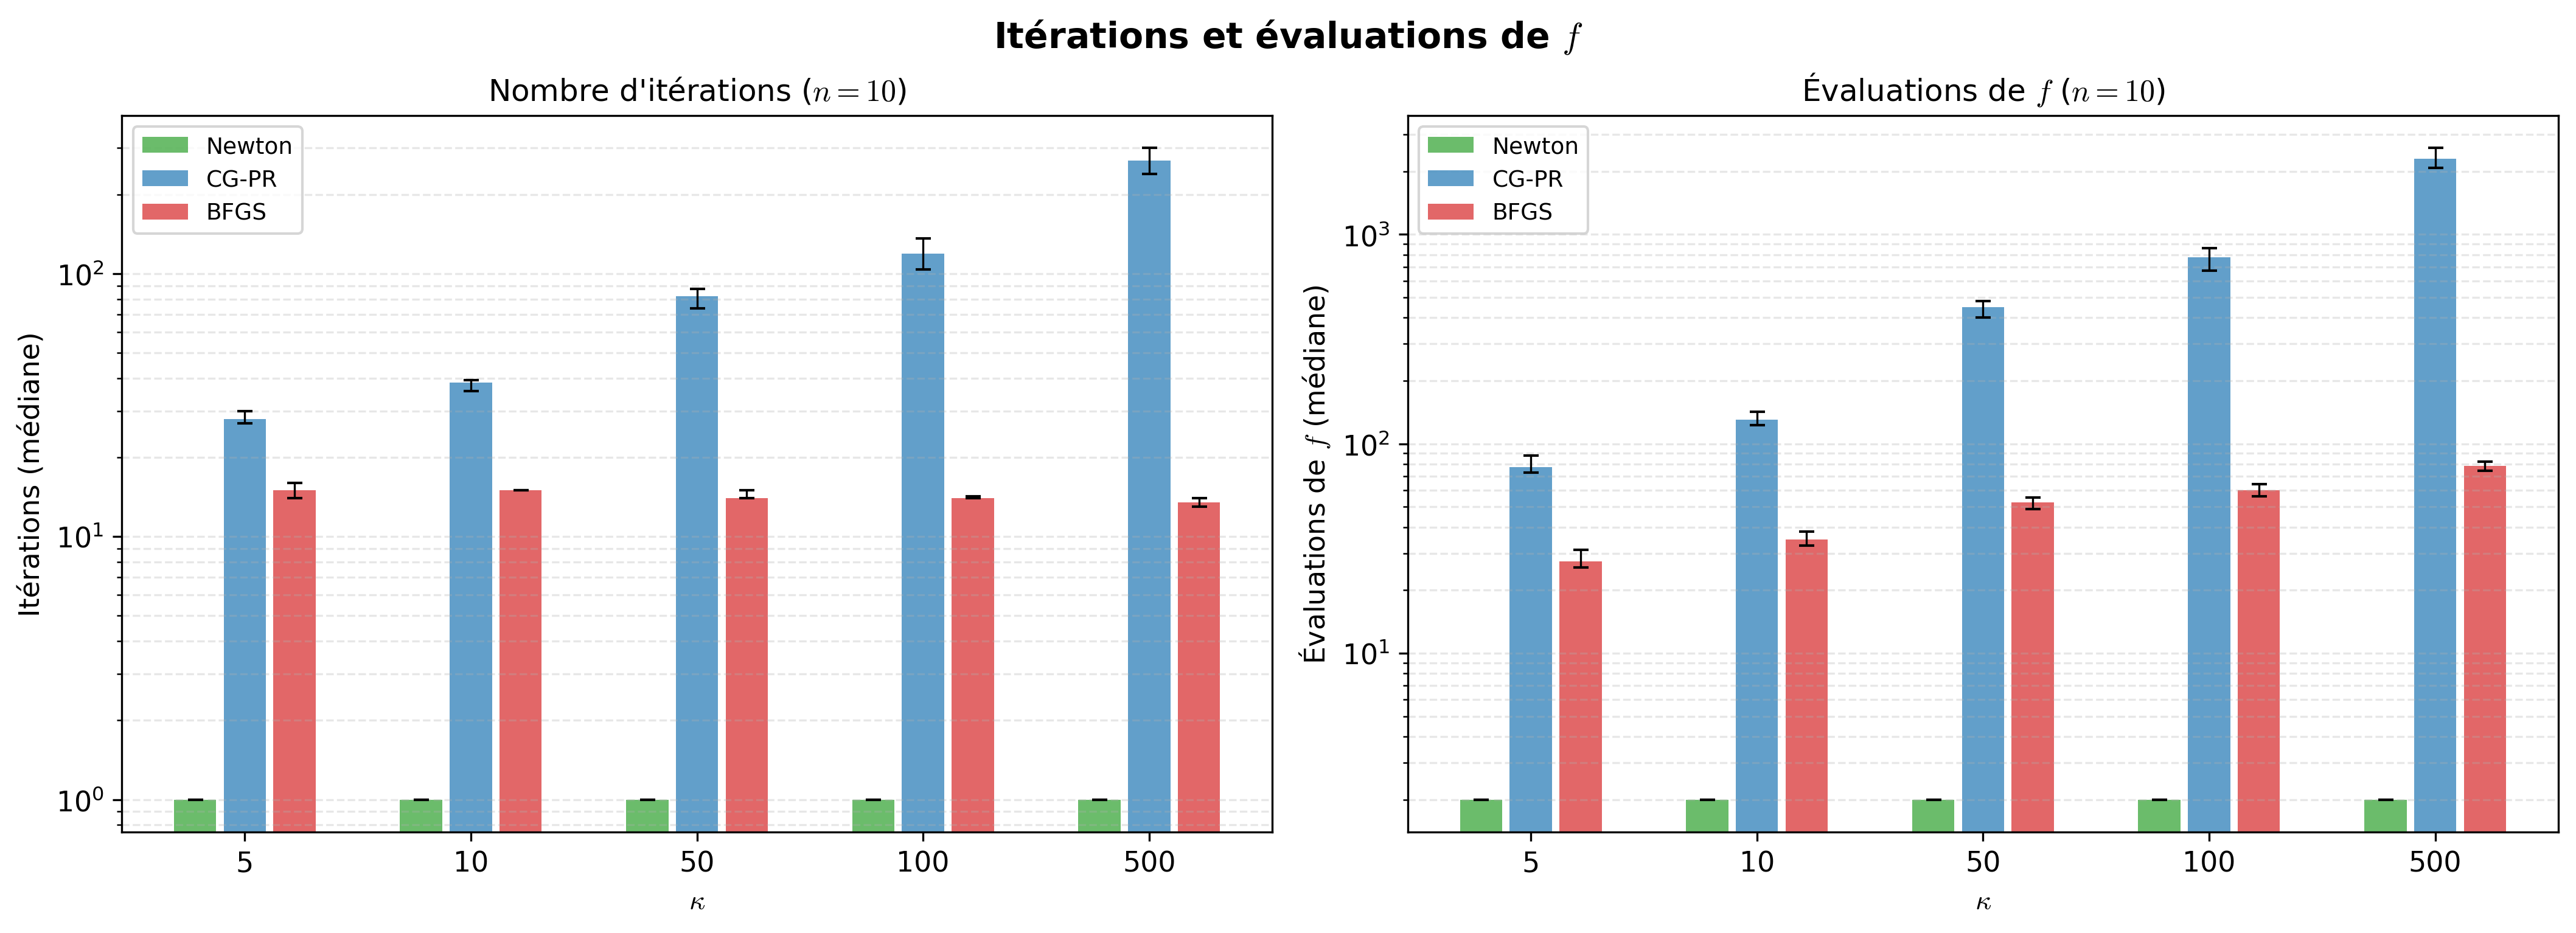
\includegraphics[width=\linewidth]{figures/benchmark3/fig5_cost.png}
  \caption{Itérations et évaluations de $f$ à $n = 10$~: coût apparent (itérations, gauche) et coût réel (évaluations de $f$, droite) en fonction de $\kappa$. Même code couleur que la figure~\ref{fig:b3_dim}.}
  \label{fig:b3_cost}
\end{figure}

La méthode de Newton n'invoque pas la recherche d'Armijo~: ses 2 évaluations de $f$ par exécution correspondent à l'évaluation initiale et à la vérification au point final. Le ratio d'évaluations de $f$ par itération de CG-PR croît avec le conditionnement, de $2.7$ à $\kappa = 50$ jusqu'à $8.6$ à $\kappa = 500$~; celui de BFGS suit la même tendance mais à un niveau inférieur, de $1.9$ à $5.8$. Le total d'évaluations de $f$ à $n = 10$ s'étale de 78 à 2298 pour CG-PR et de 28 à 78 pour BFGS. BFGS domine donc CG-PR non seulement en nombre d'itérations, mais aussi en coût réel~: il converge plus vite \emph{et} chaque itération coûte moins en évaluations de $f$ dues à la recherche d'Armijo. Cet avantage compense largement le surcoût de la mise à jour matricielle $O(n^2)$ par itération.

\paragraph{Régime général~: CG-PR contre BFGS.}
BFGS est systématiquement plus rapide que CG-PR sur les fonctions non-convexes testées (figures~\ref{fig:b3_rosen} et~\ref{fig:b3_gen_box}).

\begin{figure}[H]
  \centering
  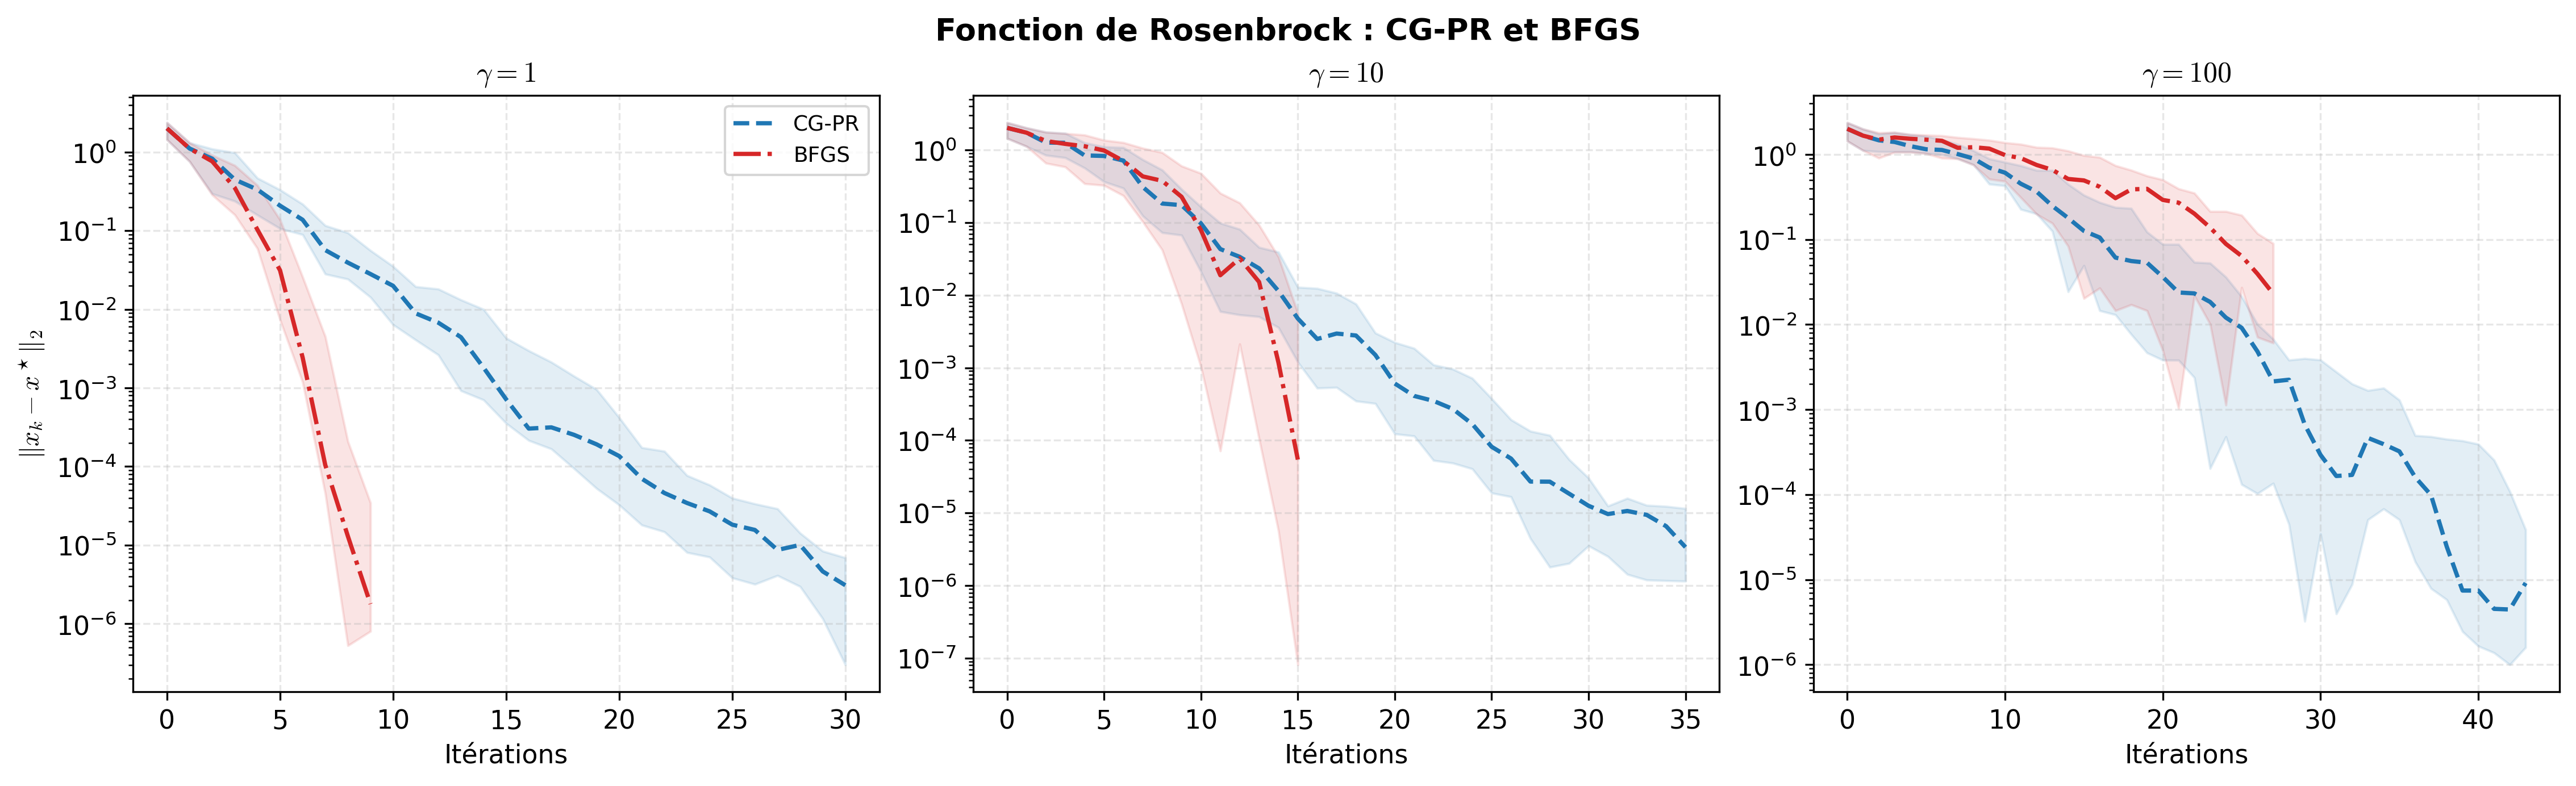
\includegraphics[width=\linewidth]{figures/benchmark3/fig6_rosenbrock.png}
  \caption{Convergence de CG-PR (bleu) et BFGS (rouge) sur la fonction de Rosenbrock~: $\|x_k - x^\star\|_2$ en fonction de $k$, médiane $\pm$ IQR sur 20 points initiaux. De gauche à droite~: $\gamma \in \{1, 10, 100\}$.}
  \label{fig:b3_rosen}
\end{figure}

\begin{figure}[H]
  \centering
  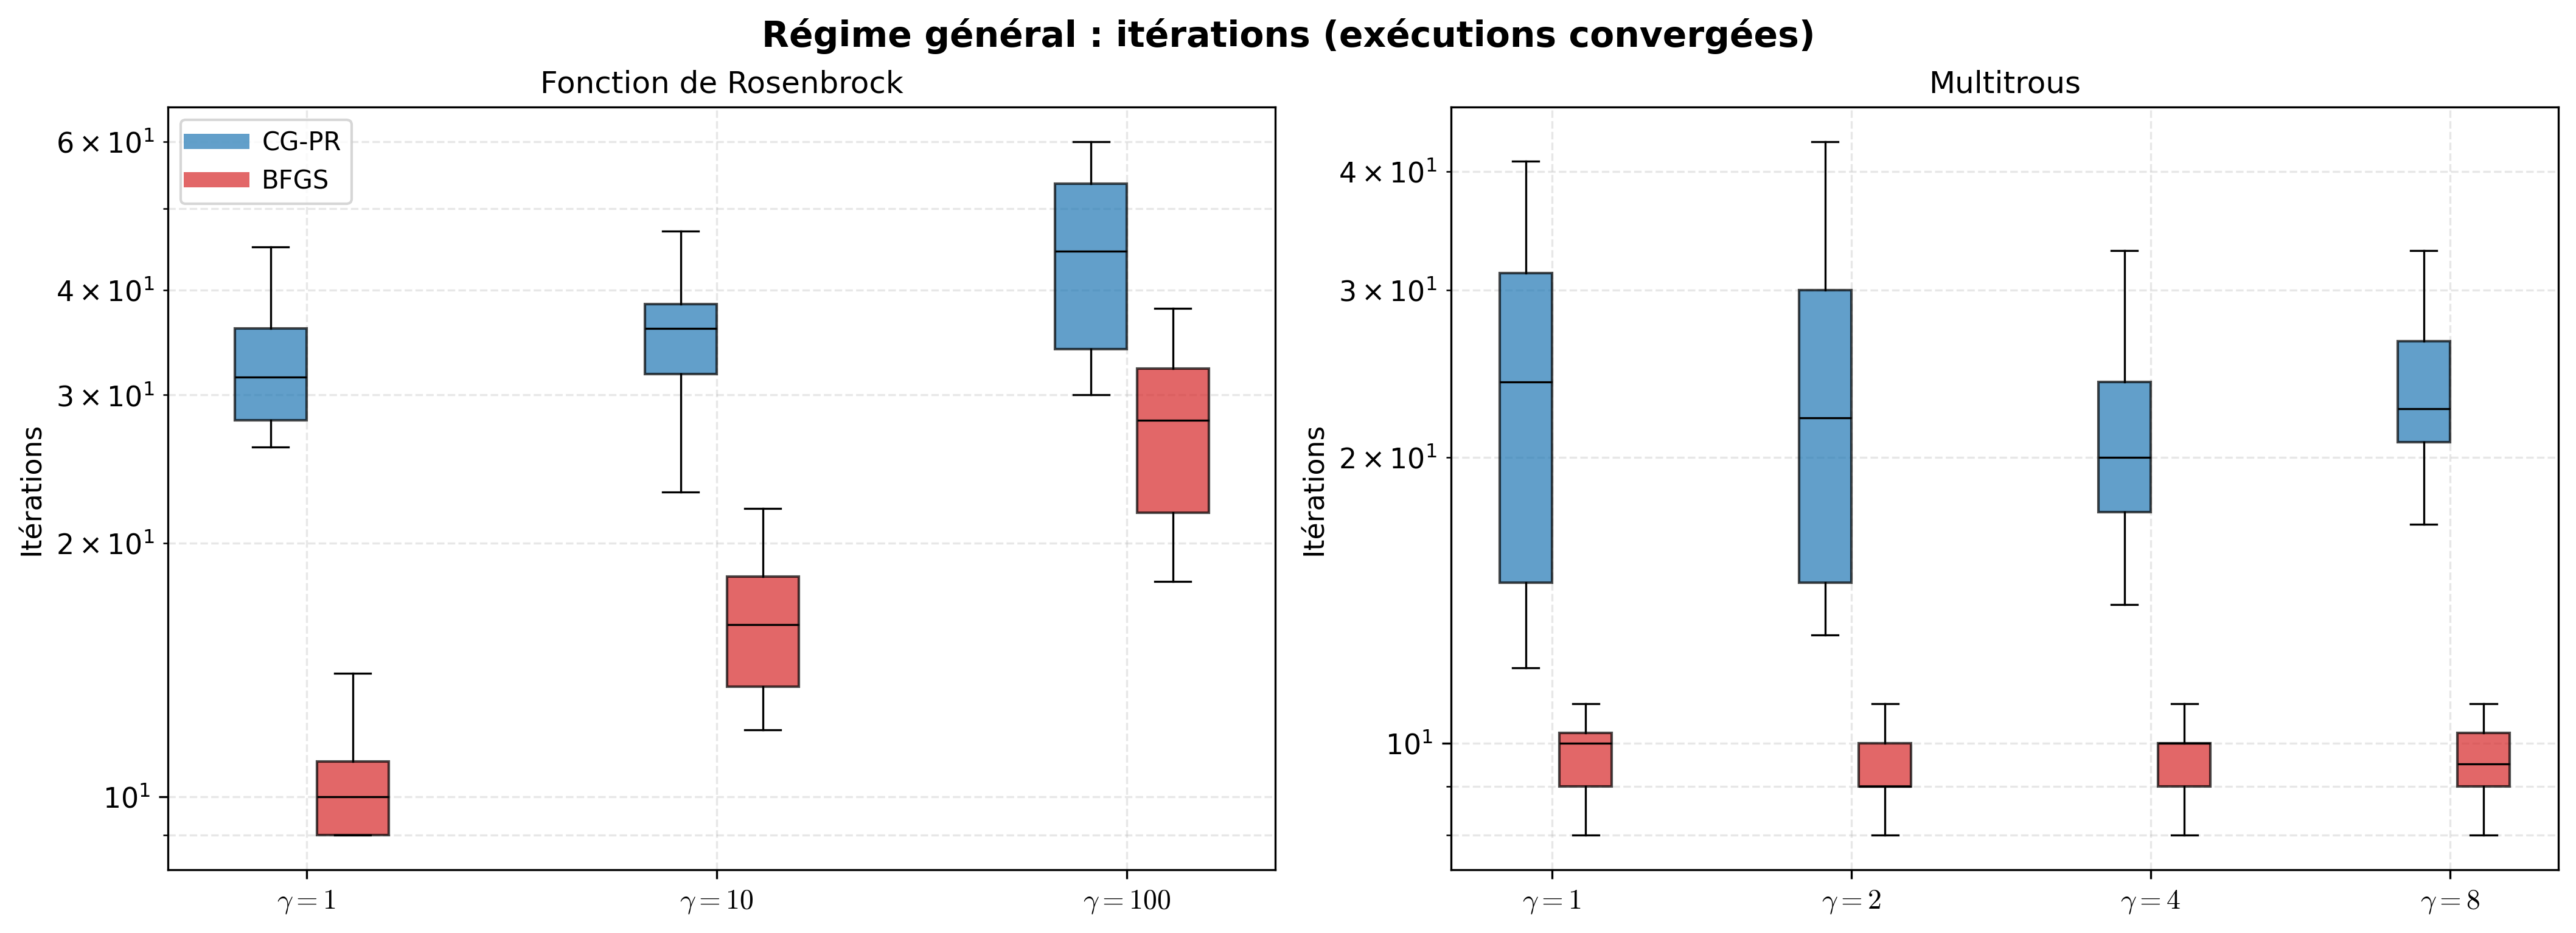
\includegraphics[width=\linewidth]{figures/benchmark3/fig7_general_iters.png}
  \caption{Distribution du nombre d'itérations parmi les exécutions convergées. CG-PR (bleu) et BFGS (rouge). Gauche~: fonction de Rosenbrock ($\gamma \in \{1, 10, 100\}$)~; droite~: fonction multitrous ($\gamma \in \{1, 2, 4, 8\}$).}
  \label{fig:b3_gen_box}
\end{figure}

Sur la fonction de Rosenbrock, les deux méthodes convergent dans $100\,\%$ des cas, mais BFGS est systématiquement plus rapide. Le ratio médian CG-PR/BFGS en itérations passe de $3.2$ à $\gamma = 1$ (32 contre 10) à $1.6$ à $\gamma = 100$ (44 contre 28)~: la vallée étroite neutralise en partie l'avantage de la direction BFGS, car les deux méthodes sont contraintes de suivre le fond de la vallée. En évaluations de $f$, l'avantage est encore plus marqué (ratio d'environ $7$ à tous les $\gamma$), car CG-PR paie un surcoût Armijo élevé sur cette géométrie.

Sur la fonction multitrous $f_M$, BFGS converge à $100\,\%$ quel que soit $\gamma$, avec une médiane de 9 à 10 itérations, contre 20 à 24 itérations pour CG-PR. CG-PR échoue sur $1$ instance sur $20$ à $\gamma = 4$ (taux de $95\,\%$), tandis que BFGS converge systématiquement ($100\,\%$ partout).

\paragraph{Synthèse.}
Les trois méthodes occupent des positions nettement distinctes dans le compromis précision-coût-robustesse. Newton exploite la structure quadratique pour converger en une itération, mais requiert l'accès explicite à $A^{-1}$ et devient inapplicable dès que la hessienne n'est plus connue. BFGS approche les performances de Newton sans calculer la hessienne~: sa convergence est super-linéaire (ordre empirique entre $1.14$ et $1.45$), quasi-insensible au conditionnement à dimension faible, et il domine CG-PR en coût réel. CG-PR offre un coût par itération plus faible ($O(n)$ contre $O(n^2)$) mais paie en nombre d'itérations et devient fragile à grande dimension ($0\,\%$ de convergence dès $n = 100$, $\kappa \geq 50$). Sur les fonctions non-convexes, BFGS conserve un avantage de facteur $1.5$ à $3$ en itérations et de facteur $\sim 7$ en évaluations de $f$ par rapport à CG-PR, avec une robustesse au moins égale.

\newpage

\section*{Conclusion}

Ce projet nous a permis de confronter systématiquement la théorie de l'optimisation numérique à la pratique expérimentale. Trois enseignements principaux se dégagent de nos benchmarks.

Premièrement, les hyperparamètres de la recherche linéaire d'Armijo ne sont pas interchangeables~: $\alpha$ et $\beta$ jouent des rôles qualitativement distincts selon la géométrie du problème, filtre de stabilité sur les vallées étroites, sélecteur de pas sur les quadratiques mal conditionnées. Le réglage de Boyd $(\alpha, \beta) = (0.25, 0.5)$ n'est pas Pareto-optimal en régime facile, mais sa robustesse en fait un choix par défaut fiable en l'absence d'information sur le problème.

Deuxièmement, la distinction entre Fletcher-Reeves et Polak-Ribière, invisible sur les fonctions quadratiques avec recherche linéaire exacte, devient déterminante en régime non-convexe. La prise en compte de la variation du gradient dans $\beta_k^{\text{PR}}$ peut contribuer à l'avantage mesuré en robustesse et en vitesse, sans nécessiter de critère heuristique supplémentaire.

Troisièmement, la hiérarchie théorique des ordres de convergence se vérifie quantitativement sur nos données~: linéaire pour le gradient conjugué, super-linéaire pour BFGS, exacte en une itération pour Newton sur les fonctions quadratiques. Ces écarts d'ordre se traduisent par des différences de coût opérationnel considérables. BFGS apparaît comme le meilleur compromis entre précision, coût et généralité parmi les méthodes testées.

Au-delà de ces résultats, ce travail illustre l'importance d'une méthodologie rigoureuse de benchmarking~: la répétition sur de nombreuses instances, la distinction entre médianes et taux de convergence, et la confrontation systématique aux bornes théoriques permettent de dépasser les observations anecdotiques et de dégager des conclusions reproductibles.

Un prolongement naturel de ce travail serait d'étendre l'analyse des bassins d'attraction du benchmark~2 à un panel plus large de méthodes~: descente de gradient, descente de plus forte pente en norme $\ell_1$, BFGS, méthodes à momentum (Nesterov, Adagrad). On pourrait alors déterminer si le choix de la méthode de descente biaise systématiquement l'optimiseur vers certains minima locaux, question à laquelle la seule comparaison FR/PR ne permet pas de répondre.

\section*{Répartition du travail}

Conformément aux attentes du projet, la charge de travail a été répartie de la manière suivante au sein de notre trinôme~:
\begin{itemize}
    \item \textbf{@KadirKess~:} Benchmark~1 (notebook, 5 figures, protocole et analyse, section~\ref{sec:b1}). Rédaction des paragraphes \emph{Descente de gradient} et \emph{Critère d'Armijo} dans la section~\ref{sec:algo}, de la section~\ref{sec:taux} et de la section~\ref{sec:arret}.
    \item \textbf{@sachaMelin~:} Benchmark~2 (notebook, 5 figures, protocole et analyse, section~\ref{sec:b2}). Rédaction de l'introduction, des sections~\ref{sec:fonctions}, \ref{sec:schema} et des paragraphes \emph{Fletcher-Reeves} et \emph{Polak-Ribière} dans la section~\ref{sec:algo}.
    \item \textbf{@valentin-best~:} Benchmark~3 (notebook, 7 figures, protocole et analyse, section~\ref{sec:b3}). Rédaction des paragraphes \emph{Méthode de Newton} et \emph{Méthode BFGS} dans la section~\ref{sec:algo}, ainsi que de la conclusion.
\end{itemize}

\end{document}